\documentclass[times, utf8, zavrsni]{fer}
\usepackage{booktabs}
\usepackage{pdfpages}
\usepackage{listings}
\usepackage{mathtools}
\usepackage{algorithmic}
\usepackage{algorithm}
\usepackage{amsmath}
\usepackage{relsize}
\usepackage[colorinlistoftodos,prependcaption,textsize=tiny]{todonotes}

\renewcommand{\lstlistingname}{Isječak}
\DeclareMathOperator*{\argmax}{arg\,max}

\begin{document}

\lstset{
    basicstyle=\linespread{1.2}\ttfamily\footnotesize,
    keepspaces=true,
    numbers=left,
    frame=single,
    showspaces=false,
    numberstyle=\ttfamily,
    columns=flexible,
    extendedchars=true,
    inputencoding=utf8,
    literate={®}{{\textregistered}}1,
}

\thesisnumber{5709}

\title{
    Sustav za određivanje strukture teksta na temelju položaja pojedinih znakova
}

\author{Herman Zvonimir Došilović}

\maketitle

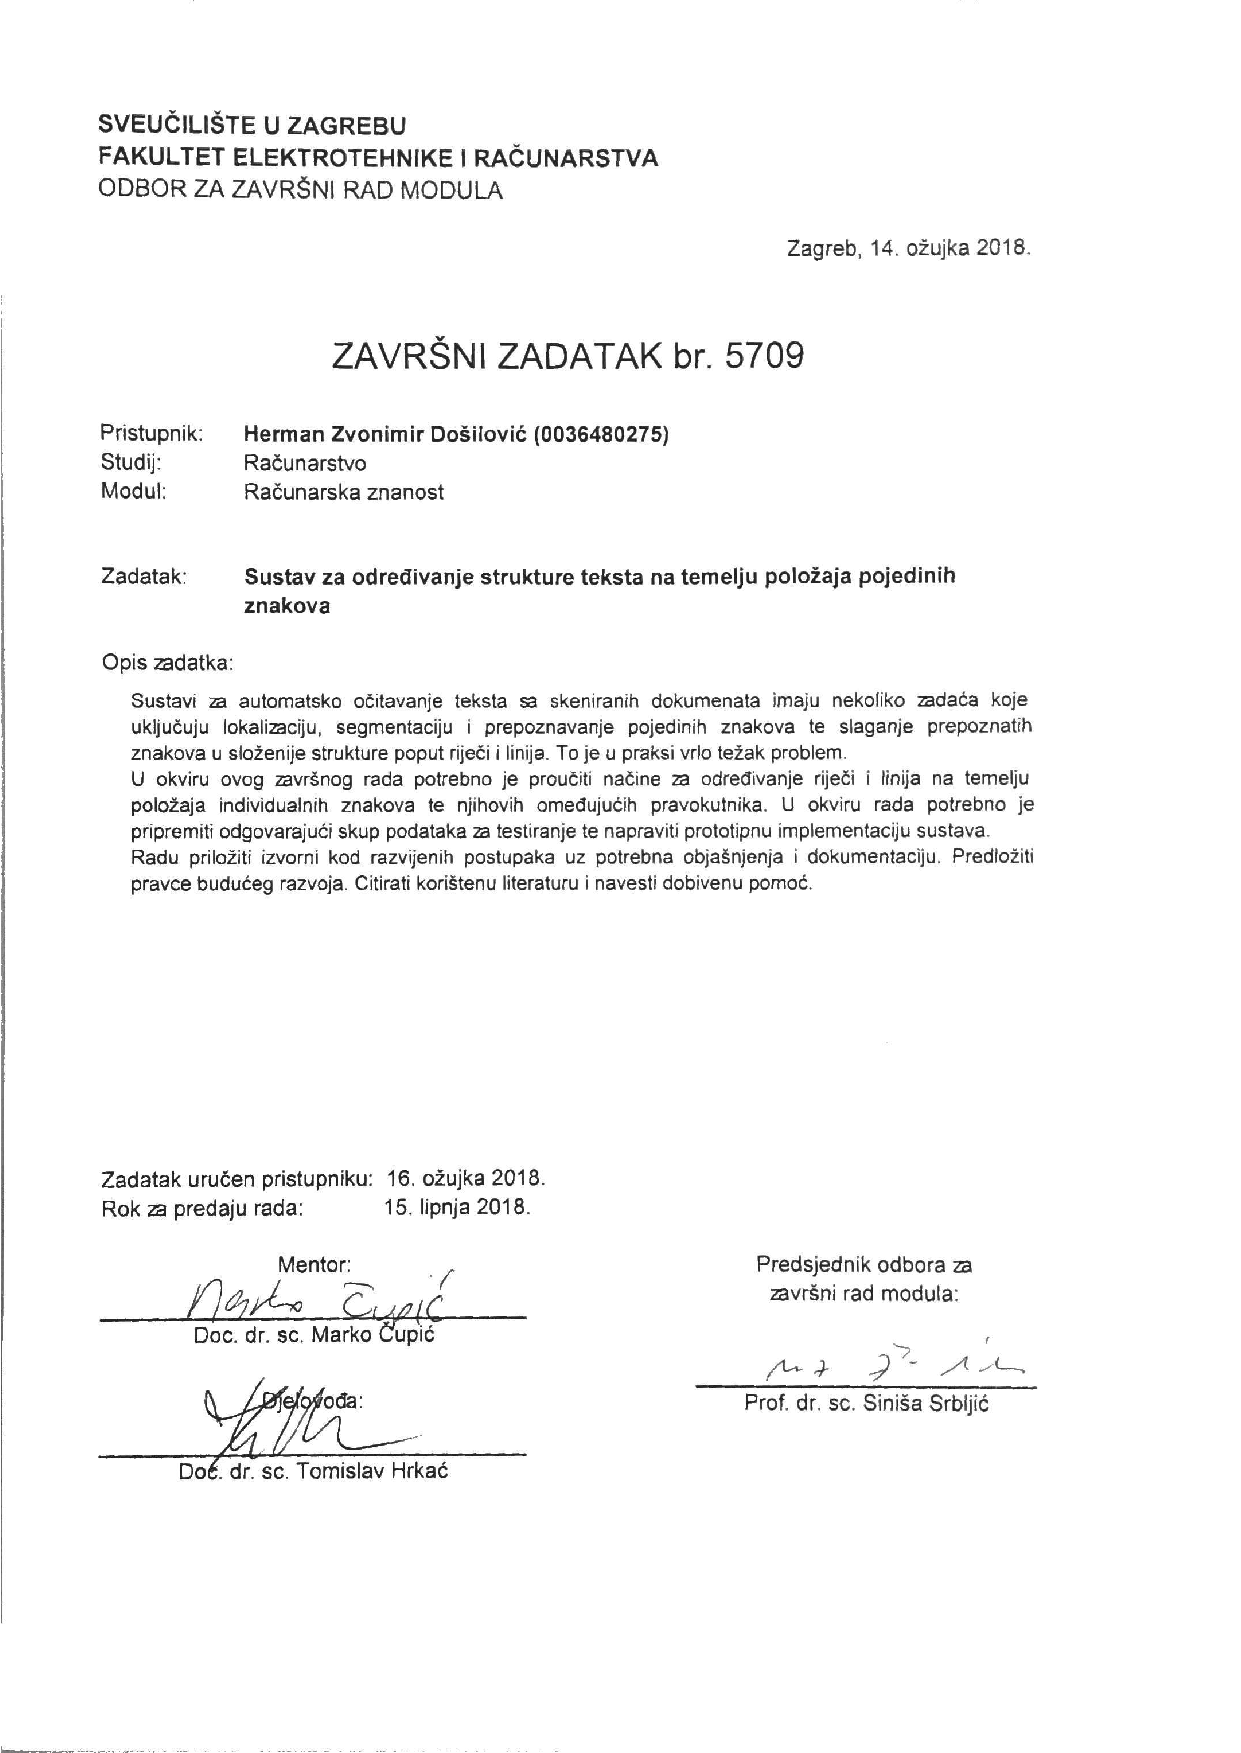
\includepdf[pages=-]{izvornik.pdf}

\zahvala{
    Zahvaljujem svom mentoru doc. dr. sc. Marku Čupiću na dozvoli za odabir
    vlastite teme i na strpljenju, poticaju i savjetima u razvoju rada.

    \

    Zahvaljujem tvrtki Microblink na danim sredstvima bez kojih ovaj rad ne bi
    bio moguć. Posebno zahvaljujem kolegama Jurici Cerovecu, Nenadu Mikši,
    Borisu Trubiću, Igoru Smolkoviču i Ivanu Jurinu koji su me svojim bogatim
    znanjem i iskustvom usmjeravali u razvoju rada.
}

\tableofcontents
















\chapter{Uvod}
Optičko raspoznavanje znakova sve je više zastupljeno u našem svakodnevnom
životu. Koristi se u provjeri osobnih dokumenata, prepoznavanju registarskih
tablica, digitalizaciji starih tiskanih knjiga, digitalizaciji raznih tiskanih
dokumenata, automatskom unosu podataka s uplatinica itd. U nekim primjenama
optičkog raspoznavanja znakova potrebna nam je i struktura očitanog sadržaja
nad kojom bi se mogla provesti daljnja analiza. Na primjer, u digitalizaciji
knjiga potrebna nam je struktura sadržaja u kojoj su znakovi grupirani u linije
i riječi kako bismo nad takvim strukturiranim sadržajem mogli provesti neku
drugu obradu. U provjeri osobnih dokumenata potrebna nam je struktura sadržaja
kako bismo mogli povratiti informacije o osobnim podacima korisnika kao što su
npr.\ njegovo ime i prezime.

Sustavi za određivanje strukture teksta sastavni su dio optičkog raspoznavanja
znakova. U ovom završnom radu predložit ćemo nekoliko načina za određivanje
strukture teksta koji će u nestrukturiranom sadržaju odrediti linije i riječi
samo na temelju položaju pojedinih znakova. Sustav za određivanje strukture
teksta na temelju položaja pojedinih znakova, implementiran u skopu ovog rada,
rješavat će problem određivanje strukture teksta u sadržaju s računa iz
trgovine i u sadržaju iz knjiga. Sustav će biti podjeljen na dva podsustava od
kojih će prvi odrediti linije, a drugi će rastaviti riječi u svakoj liniji.

U drugom poglavlju opisane su primjene i način rada sustava za optičko
raspoznavanje znakova. Treće poglavlje daje uvid u dosadašni rad u području
određivanja strukture teksta, a četvrto poglavlje detaljno opisuje problem koji
rješava ovaj rad. Također, u okviru četvrtog poglavlja bit će opisan skup
podataka za testiranje razvijenog sustava. Poglavlje
\ref{chap:algoritmi-za-odredivanje-strukture-teksta} formalno opisuje način rada
algoritama za određivanje linija i algoritama za rastavljanje riječi koji
zajedno čine sustav za određivanje strukture teksta. Rezultati i analiza
algoritama, kao i korištene mjere točnosti opisane su u šestom poglavlju. U
sklopu analize dane su smjerince za budući rad.
















\chapter{Optičko raspoznavanje znakova}
\label{chap:opticko-raspoznavanje-znakova}
Sustav za optičko raspoznavanje znakova \engl{optical character recognition} (u
daljnjem tekstu: \emph{OCR-sustav})
pretvara sliku tiskanog teksta u digitalizirani format kojim možemo jednostavno
manipulirati na računalu.
Iako je to ljudima jednostavan zadatak, računalima nije lako prepoznati tekst i
pojedine znakove teksta sa slike
zbog velike raznolikosti jezika, fonta i stila kojim tekst može biti napisan.
Optičko raspoznavanje znakova je stoga vrlo zahtjevan problem i mnogo je
istraživačkog truda uloženo u pokušaju
da se slike teksta pretvore u format koji računalo razumije. \citep
{DBLP:journals/corr/abs-1710-05703}









\section{Primjene}
Osim tiskanog teksta, OCR-sustavi koriste se i u prepoznavanju znakova rukom
pisanog teksta. Prepoznavanje znakova rukom pisanog teksta je teži problem od
prepoznavanja tiskanog teksta \citep{DBLP:journals/corr/abs-1710-05703} zato jer
se oblik znakova i njihov način pisanja razlikuje kod svake osobe (npr.\
rukopis odrasle osobe potpuno je drugačiji od rukopisa djeteta).
OCR-sustave za detekciju rukom pisanih znakova možemo podijeliti na dvije
potkategorije: \emph{on-line} i \emph{off-line}. \emph{On-line} OCR-sustavi
detektiraju znakove dok ih korisnici unose i to im omogućuje praćenje
parametara poput: brzine pisanja, broja napravljenih poteza,
smjer pisanja, itd. \emph{Off-line} OCR-sustavi izvode se nad jednom slikom na
kojoj se nalazi sav sadržaj nad kojim je potrebno napraviti detekciju. Takvi
sustavi nemaju dodatne informacije koje imaju \emph{on-line} sustavi i zato je
detekcija znakova kompliciranija \citep{DBLP:journals/corr/abs-1710-05703}.
Slika \ref{fig:math-example-01} prikazuje primjer rezultata \emph{off-line}
OCR-sustava za detekciju rukom pisanih znakova. OCR-sustavi imaju široku
primjenu i možemo ih pronaći primjerice u detekciji znakova na registarskim
pločicama \citep{DBLP:journals/corr/Saghaei16a},
\citep{DBLP:journals/corr/abs-1802-09567}, u detekciji znakova sadržaja knjiga
\citep{DBLP:journals/corr/abs-1802-10033},
\citep{Christy:2017:MDE:3172938.3075645} i detekciji znakova na raznim
dokumenatima \citep{DBLP:journals/corr/HarrajR15} \citep{verma2016ocr}. Na
slici \ref{fig:receipt-example-01} prikazan je primjer rezultata korištenja
OCR-sustava za detekciju znakova na računima iz trgovine. Slika
\ref{fig:book-example-01} prikazuje rezultat OCR-sustava za detekciju znakova
na tiskanim knjigama.

\pagebreak

\begin{figure}[htb]
    \centering
    \captionsetup{justification=centering,margin=2cm}
    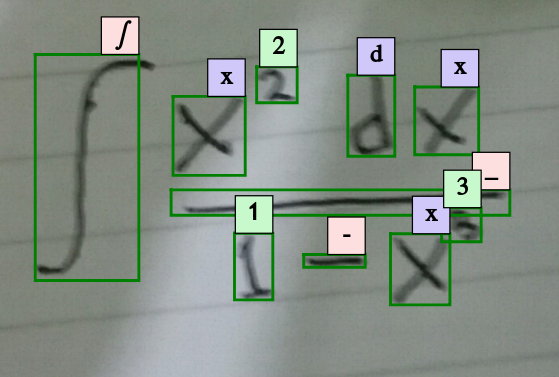
\includegraphics[height=4cm]{images/math-example-01.png}
    \caption{
        Rezultat \emph{off-line} OCR-sustava za detekciju znakova rukom pisanog
        teksta.
    }
    \label{fig:math-example-01}
\end{figure}

\begin{figure}[htb]
    \centering
    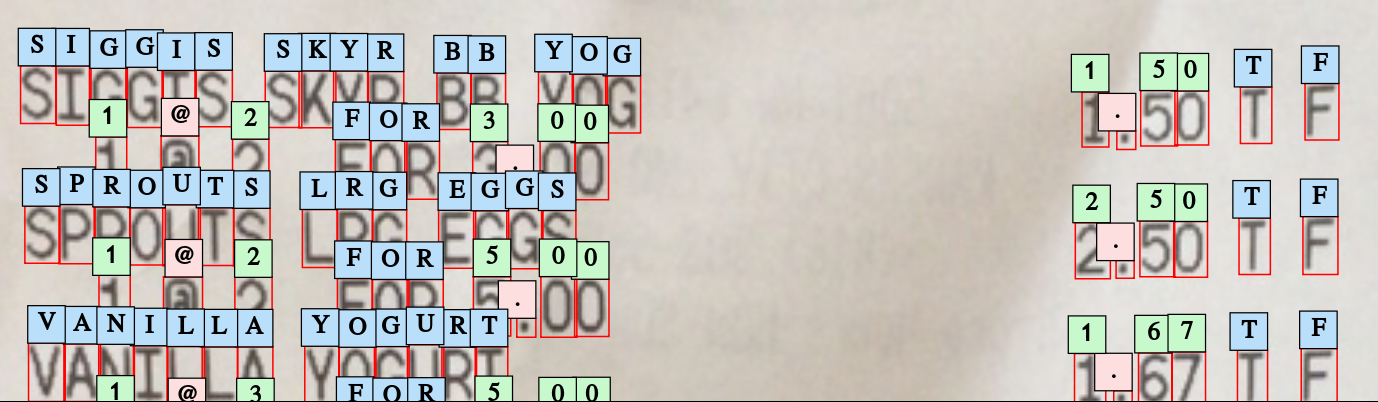
\includegraphics[width=\textwidth]{images/receipt-example-01.png}
    \caption{Rezultat OCR-sustava za detekciju znakova na računima iz trgovine.}
    \label{fig:receipt-example-01}
\end{figure}

\begin{figure}[htb]
    \centering
    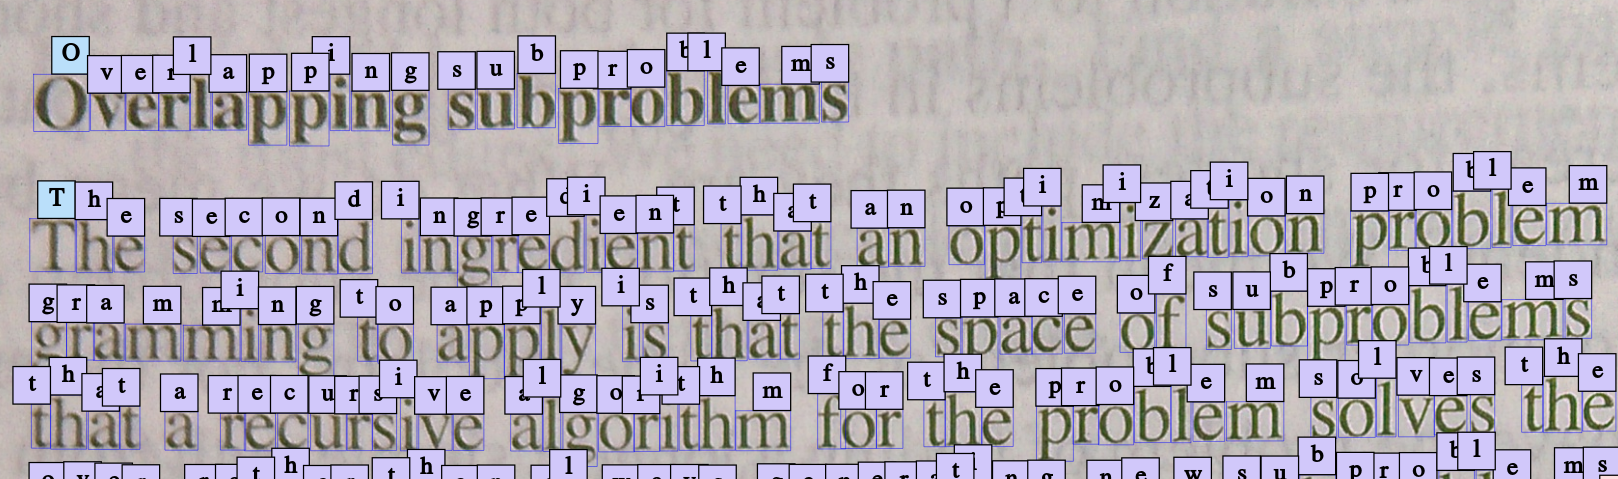
\includegraphics[width=\textwidth]{images/book-example-01.png}
    \caption{Rezultat OCR-sustava za detekciju znakova na tiskanim knjigama.}
    \label{fig:book-example-01}
\end{figure}

\pagebreak








\section{Komponente OCR-sustava}
\label{sec:komponente-ocr-sustava}
Optičko raspoznavanje znakova provodi se u nekoliko koraka
\citep{DBLP:journals/corr/abs-1710-05703} \citep{kaur2016survey}:

\begin{enumerate}
    \item pribavljanje slike,
    \item predobrada,
    \item segmentacija znakova,
    \item izdvajanje značajki znakova,
    \item klasifikacija znakova i
    \item naknadna obrada.
\end{enumerate}


\subsubsection{Pribavljanje slike}
U prvom koraku OCR-a, pribavljanju slike, potrebno je pribaviti sliku nad kojom
ćemo provesti ostale korake. Sliku možemo pribaviti s raznih uređaja poput
kamere fotoaparata, mobilnog uređaja ili nekog drugog uređaja za digitalizaciju
dokumenata \engl{scanner}. Nakon prvog koraka, slika dokumenta nad kojim
provodimo raspoznavanje znakova sastoji se samo od slikovnih elemenata
\engl{pixels} \citep{Vynckier:2018:HowOcrWorks}. Slika
\ref{fig:receipt-example-02} prikazuje primjer slike nad kojom možemo provesti
postupak raspoznavanja znakova. Slika može sadržati pozadinu koju
bi OCR-sustav trebao zanemariti.

\

\begin{figure}[htb]
    \centering
    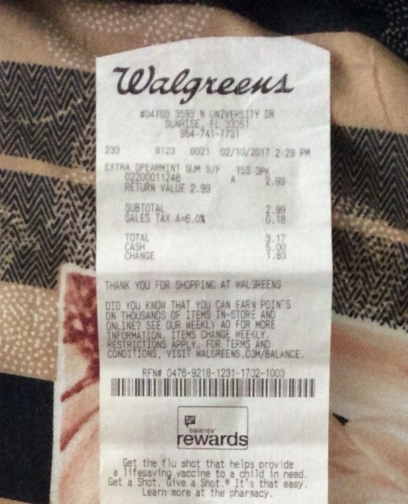
\includegraphics[height=6.3cm]{images/receipt-example-02.jpeg}
    \caption{Ulazna slika u OCR-sustav pribavljena kamerom mobilnog uređaja.}
    \label{fig:receipt-example-02}
\end{figure}


\subsubsection{Predobrada}
U predobradi slike OCR-sustavi često provode niz morfoloških transformacija i
filtra nad pribavljenom slikom. Cilj ovog koraka je povećati kvalitetu slike i
smanjiti informacije na slici. Binarizacija je jedan od potkoraka predobrade
koji slike u boji ili u nijansama sive pretvara u crno-bijele. Osim binarizacije
koriste se neke morfološke transformacije poput dilatacije, rezanja i
skaliranja. Slika \ref{fig:binarization} prikazuje primjer slike prije i nakon
binarizacije. \citep{Gulan:2016:Bacherlor},
\citep{DBLP:journals/corr/abs-1710-05703}, \citep{Jurin:2017:Master}

\

\begin{figure}[htb]
    \centering
    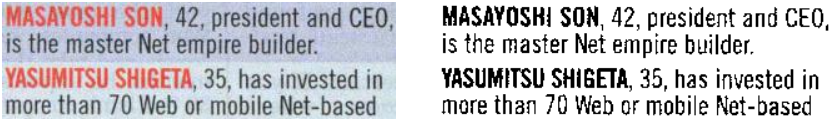
\includegraphics[width=\textwidth]{images/binarization.png}
    \caption{
        Prije binarizacije (lijevo) i nakon binarizacije (desno)
        \citep{Vynckier:2018:HowOcrWorks}.
    }
    \label{fig:binarization}
\end{figure}


\subsubsection{Segmentacija znakova}
\label{subsubsec:segmentacija}
Sljedeći korak, segmentacija znakova, je postupak segmentiranja slike u
segmente unutar kojih se nalaze znakovi koje želimo klasificirati. Jedan od
pristupa segmentacije izvodi se s vrha prema dnu gdje se prvo segmentiraju
linije, zatim riječi i na kraju pojedini znakovi \citep{Jurin:2017:Master},
\citep{Vynckier:2018:HowOcrWorks}. Prednost ovakvog pristupa je da uz lokaciju
svakog znaka dobivamo i strukturu cijelog teksta, odnosno, znamo kojoj liniji i
kojoj riječi znak pripada. Nedostatak ovakvog pristupa je da ne postoje
korekcijski mehanizmi kojima bismo znak pridružili nekoj drugoj liniji ili
riječi ako su prva dva koraka segmentacije linije ili riječi neispravni.
\citep{Jurin:2017:Master}

Drugi pristupi poput \emph{ZICER OCR}\footnote{OCR-sustav tvrtke
\emph{Microblink}, \url{https://microblink.com}} sustava izravno
izvode segmentaciju cijele slike na području koji predstavljaju znakove.
Prednost takvog pristupa je da možemo detektirati znakove teksta u kojemu nema
riječi i linija, kao što je na primjer matematički izraz. Nedostatak takvog
pristupa je da gubimo informaciju o strukturi teksta i zato postoji potreba za
razvojem dodatnog sustava koji bi znakove grupirao u riječi, a riječi u linije
\citep{Jurin:2017:Master}. Slika \ref{fig:segmentation} prikazuje rezultat
segmentacije pojedinih znakova.

\begin{figure}[htb]
    \centering
    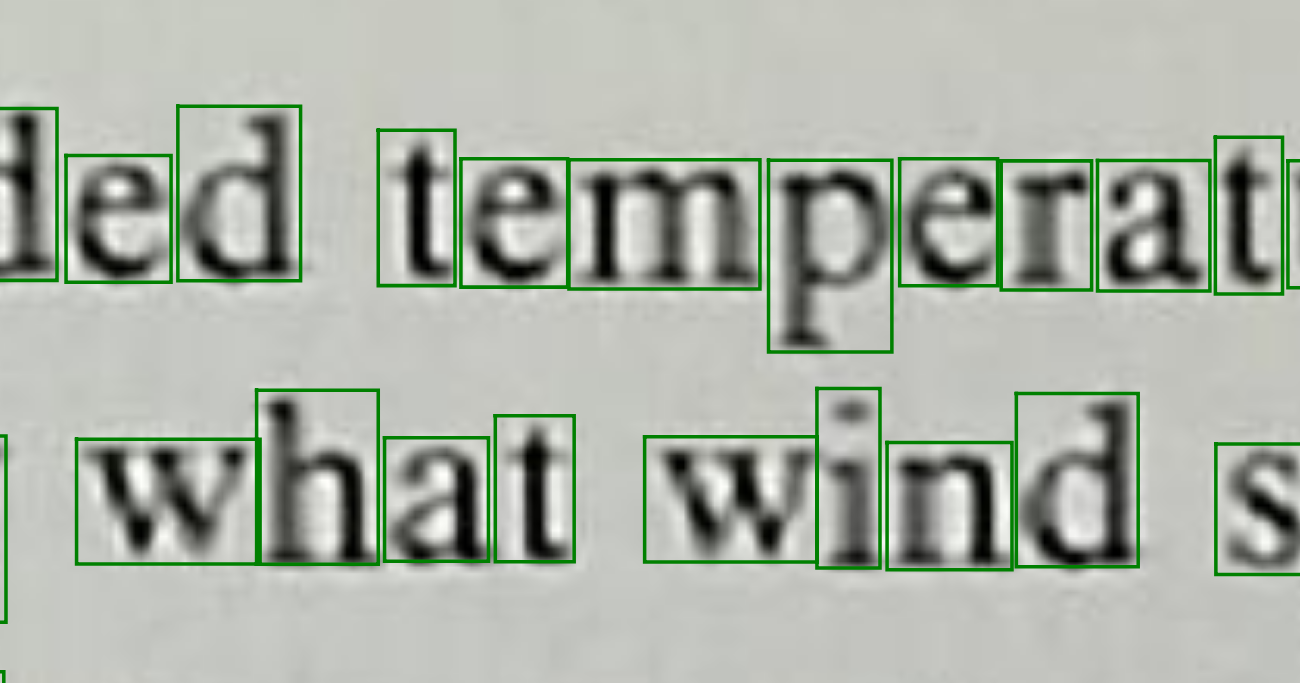
\includegraphics[height=4cm]{images/segmentation.png}
    \caption{Segmentacija znakova.}
    \label{fig:segmentation}
\end{figure}

\pagebreak

\subsubsection{Izdvajanje značajki}
Izdvajanje značajki pojedinog znaka podrazumijeva odabir značajki prema kojima
će se jedinstveno klasificirati svaki znak. Značajke poput geometrijskog oblika
ili statističkih svojstava mogu biti uzete u obzir prilikom klasifikacije.
Važno područje istraživanja pripada razmatranju koje i koliko značajki je
potrebno uzeti u obzir za kvalitetnu i ispravnu klasifikaciju.
\citep{DBLP:journals/corr/abs-1710-05703}


\subsubsection{Klasifikacija}
Klasifikacija je najvažniji korak optičkog raspoznavanja znakova
\citep{verma2012survey} \citep{zhu2016novel} koji koristi izdvojene značajke za
određivanje klase pojedinog znaka \citep{lehal1999feature}
\citep{kaur2016survey}. Statistički pristupi klasifikacije koriste
diskriminativne funkcije za određivanje klase znaka
\citep{DBLP:journals/corr/abs-1710-05703}, a u novije vrijeme koriste se duboke
neuronske mreže \citep{Jurin:2017:Master}. Neki od statističkih pristupa su:
Bayesov klasifikator, klasifikator stablom odluke, umjetne neuronske mreže i
metoda k-najbližih susjeda \citep{DBLP:journals/corr/abs-1710-05703}.

\citep{krizhevsky2012imagenet} objavili su rad koji je označio prekretnicu u
klasifikaciji i lokalizaciji objekata \citep{Jurin:2017:Master}. Slika
\ref{fig:deep-example-01} prikazuje arhitekturu \emph{AlexNet} koja je
pobijedila na natječaju \emph{ImageNet 2012} u području klasifikacije objekata.
\citep{Jurin:2017:Master}

\begin{figure}[!htb]
    \centering
    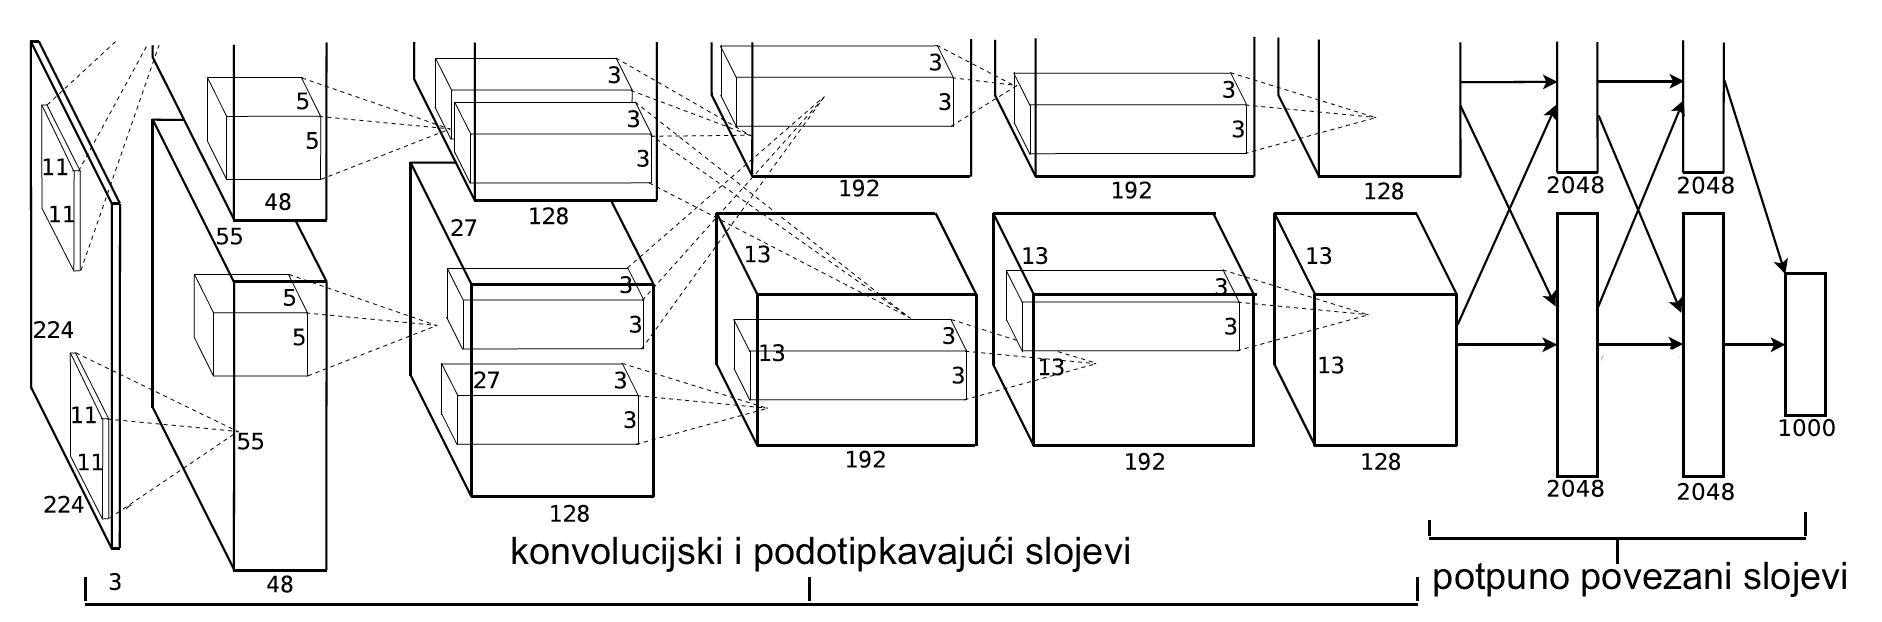
\includegraphics[height=4.2cm]{images/deep-example-01.png}
    \caption{Arhitektura \emph{AlexNet} \citep{Jurin:2017:Master}.}
    \label{fig:deep-example-01}
\end{figure}


\subsubsection{Naknadna obrada}
Nakon klasifikacije znakova slijedi njihova naknadna obrada koja se koristi kako
bi se poboljšali OCR-rezultati. Jedan od pristupa postprocesiranja koristi
rezultate više različitih klasifikatora koji mogu biti korišteni slijedno,
paralelno ili hijerarhijski. Nakon toga rezultati klasifikatora se kombiniraju
različitim pristupima \citep{DBLP:journals/corr/abs-1710-05703}. Kao što je
prije spomenuto, segmentacija koja se ne provodi s vrha
prema dnu nema informaciju o strukturi teksta i zato je potrebno razviti dodatan
\textbf{sustav za određivanje strukture teksta na temelju položaja pojedinih
znakova}.

\citep{schulz2017multi} predstavili su arhitekturu
tzv. \emph{post-correction} OCR-sustava kojim su pokazati na koji su način
adaptirali generički sustav za naknadnu obradu OCR-rezultata koristeći domensko
znanje za konkretan problem koji su rješavali. Ovim pristupom ostvarili su bolje
rezultate za konkretni problem nego što su ostvarili koristeći postojeći
generički sustav za naknadnu obradu OCR-rezultata.

\

\begin{figure}[htb]
    \centering
    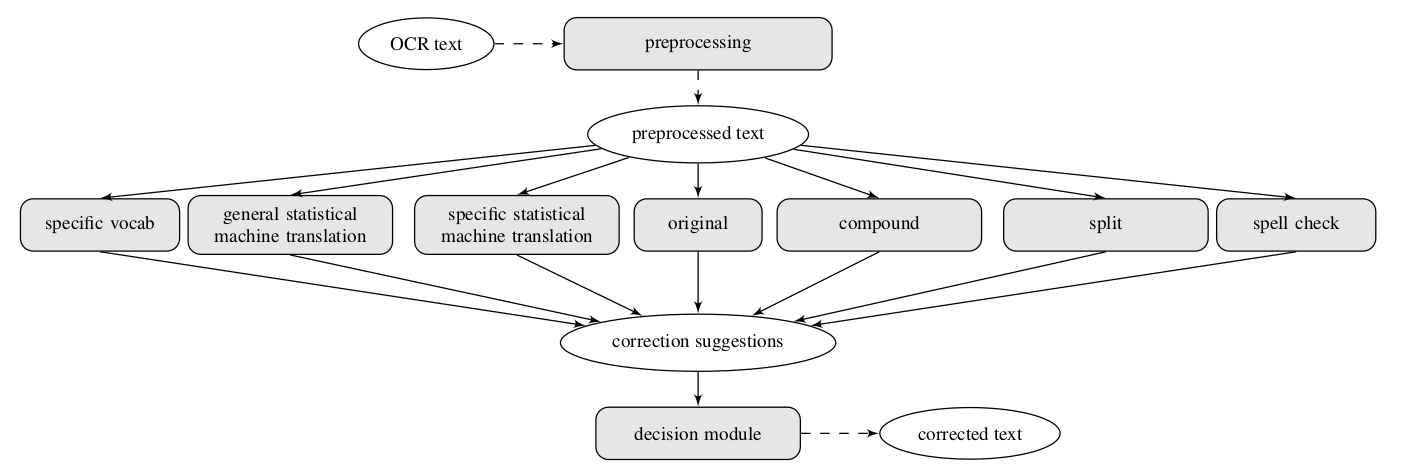
\includegraphics[width=\textwidth]{images/post-correction-example-01.png}
    \caption{
        Arhitektura \emph{post-correction} OCR sustava \citep{schulz2017multi}.
    }
    \label{fig:post-correction-example-01}
\end{figure}
















\chapter{Određivanje strukture teksta}
Sustavi za određivanje strukture teksta na temelju OCR-rezultata sastavni su
dio OCR-sustava. Određivanje strukture teksta podrazumijeva segmentaciju linija
i segmentaciju riječi unutar linije. Neke tehnike segmentacije znakova i
njihove klasifikacije nemaju informaciju o tome kojoj liniji i riječi pojedini
znak pripada. Prednost takvog pristupa je da takav OCR-sustav možemo koristiti
nad slikama koje ne sadrže linije, kao što su na primjer slike matematičkih
izraza \citep{Jurin:2017:Master}. Nedostatak je što nakon klasifikacije moramo
razviti sustav koji će znakove naknadno obraditi da bismo odredili strukturu
teksta \citep{Jurin:2017:Master}.

Tekst na slici može biti podijeljen na linije ili blokove, a u bloku tekst
možemo podijeliti na linije. Unutar jedne linije znakove možemo grupirati u
riječi. Način na koji će se odrediti struktura teksta uvelike ovisi o problemu
koji rješavamo i kakve rezultate želimo dobiti. Tekst na slici
\ref{fig:text-segmentation-01} podijeljen je na linije (plavo), a unutar svake
linije na riječi (crveno).

\begin{figure}[htb]
    \centering
    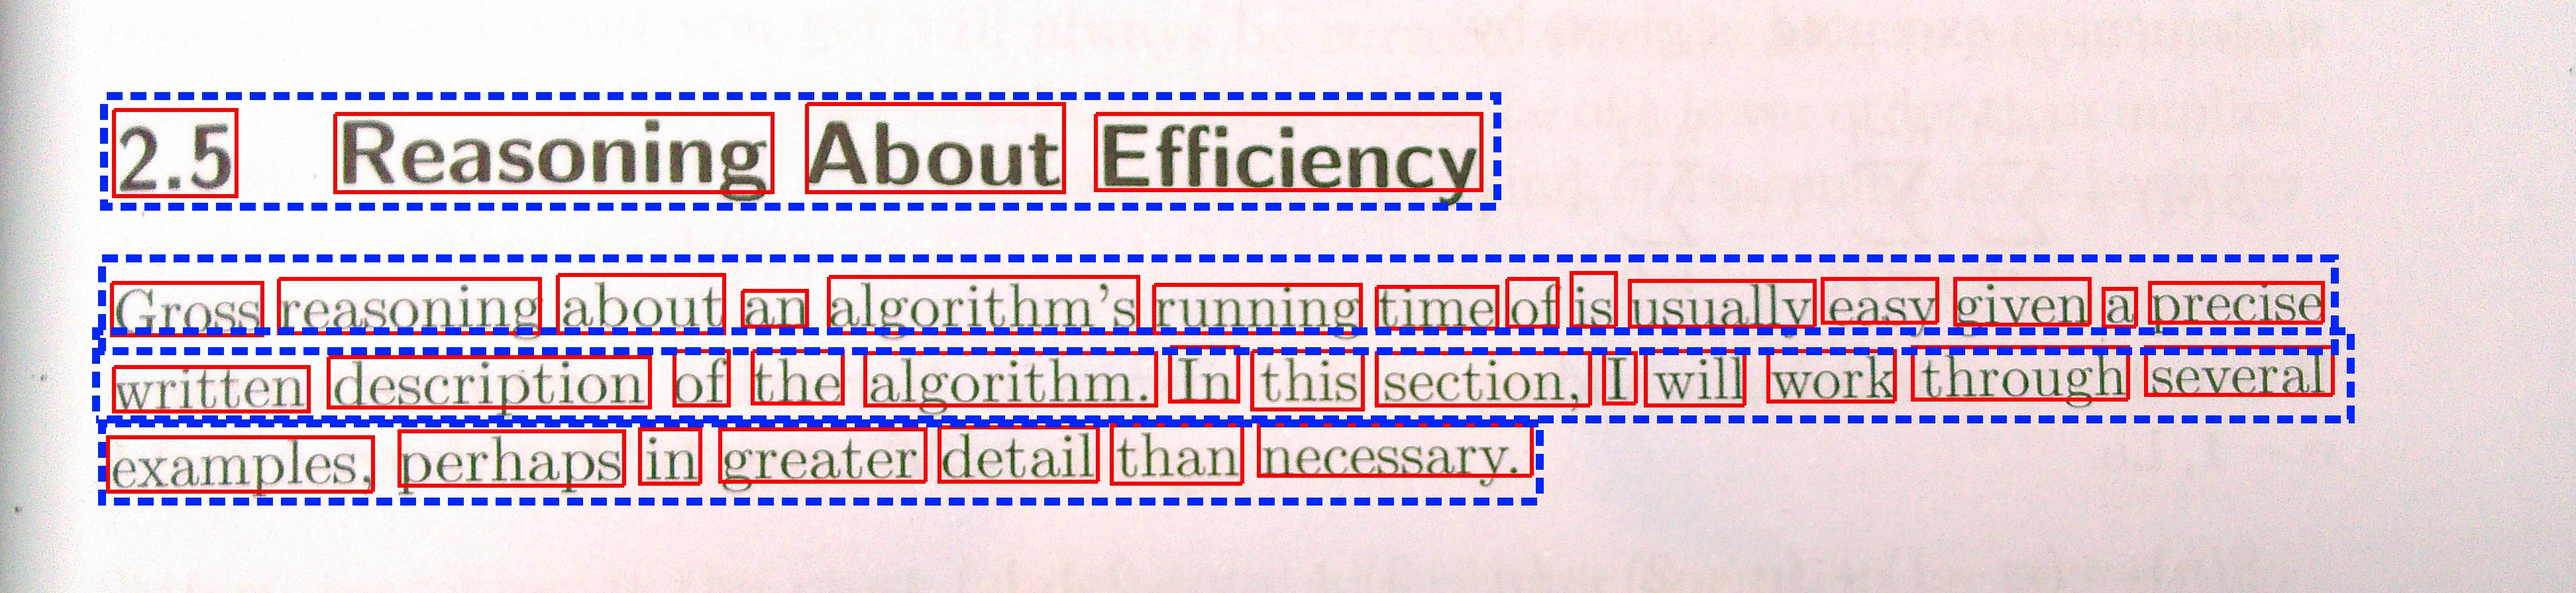
\includegraphics[width=\textwidth]{images/text-segmentation-01.jpg}
    \caption{Segmentacija linija (plavo) i riječi (crveno) unutar linije.}
    \label{fig:text-segmentation-01}
\end{figure}

\citep{DBLP:journals/corr/TianPHLYT16} predložili su sustav za određivanje
strukture teksta koji će osim određivanja kojoj liniji pojedini znak pripada
znati izbaciti tzv. \emph{false positive} znakove odnosno znakove koje je
OCR-sustav prepoznao, a zapravo u tekstu ne postoje. Njihov sustav temelji
se na \emph{min-cost flow network} modelu koji objedinjuje izbacivanje
\emph{false positive} znakova i pronalazak strukture teksta. Na temelju
međusobne pozicije između dva prepoznata znaka i dodatnog parametra kojeg
dobivaju od klasifikatora, a koji označava vjerojatnost ispravne detekcije,
grade težinski usmjereni graf (slika \ref{fig:text-flow}).

\begin{figure}[htb]
    \centering
    \captionsetup{justification=centering}
    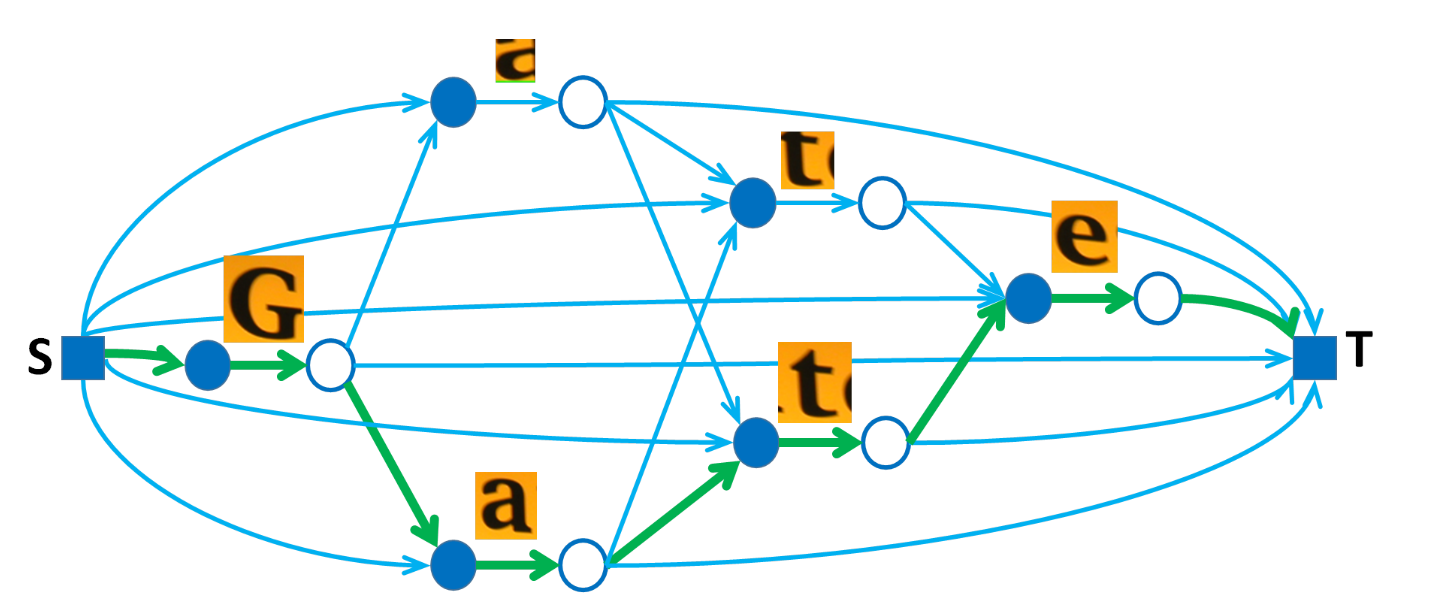
\includegraphics[height=6cm]{images/text-flow.png}
    \caption{Težinski usmjereni graf \citep{DBLP:journals/corr/TianPHLYT16}.}
    \label{fig:text-flow}
\end{figure}

\citep{zhu2016novel} predložili su novu arhitekturu (slika \ref{fig:novel-ocr})
OCR-sustava koji se temelji na empirijskim rezultatima koji su pokazali da
sadržaj riječi ne ovisi samo o dijelu teksta u kojem se ta riječ nalazi nego i
o susjednim dijelovima teksta. Njihov OCR-sustav radi dvostruku analizu
strukture teksta -- prije klasifikacije i nakon klasifikacije. Prva analiza
strukture teksta omogućuje im da odrede strukturu teksta u blokovima, a druga
analiza strukture teksta im omogućuje da poprave pogreške u klasifikaciji.
Njihova nova arhitektura predstavlja hibridni OCR-sustav koji iskorištava
rezultate analize strukture teksta.

\

\begin{figure}[htb]
    \centering
    \captionsetup{justification=centering}
    \fbox{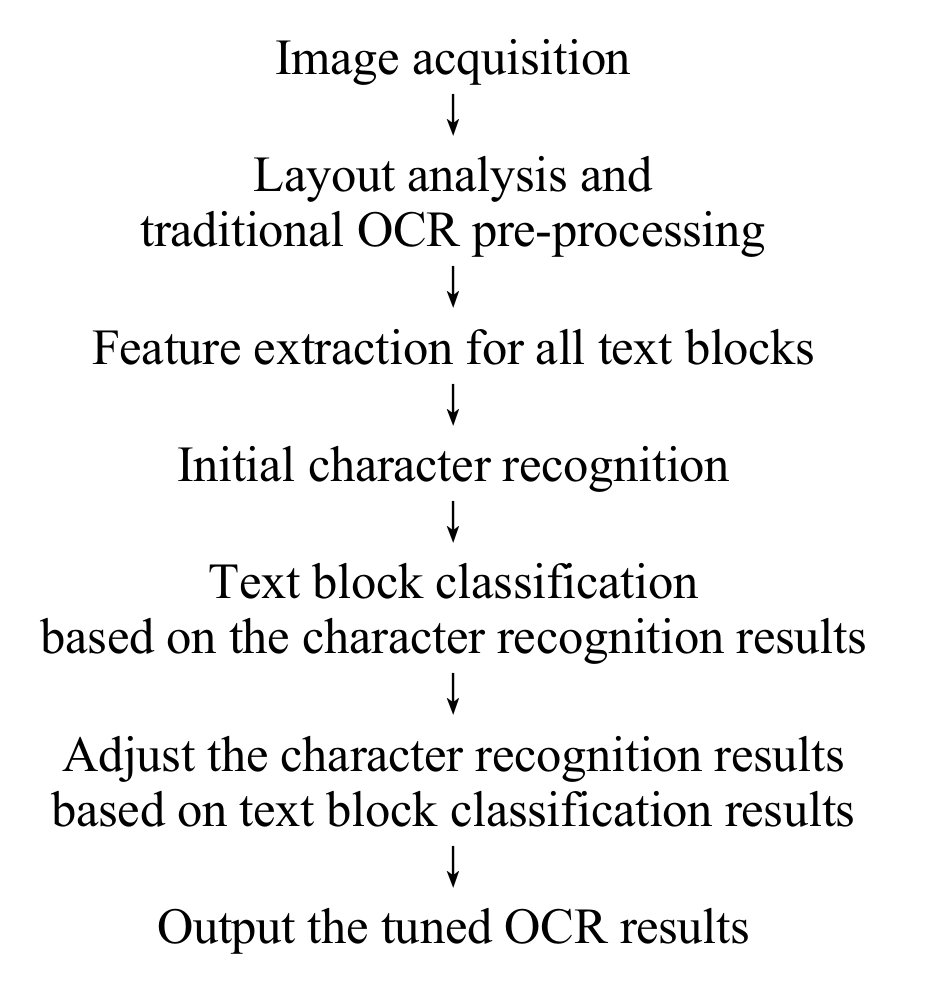
\includegraphics[height=7cm]{images/novel-ocr.png}}
    \caption{Arhitektura OCR-sustava kojeg predlažu \citep{zhu2016novel}.}
    \label{fig:novel-ocr}
\end{figure}

\pagebreak

\citep{yin2007handwritten} pronalaze linije u tekstu povezujući znakove u
težinski graf nad kojim provode Kruskalov algoritam za pronalazak minimalnog
razapinjujućeg stabla. Njihov pristup ne koristi rezultate klasifikacije, nego
koriste povezane komponente koje im predstavljaju znakove i koje pronalaze
koristeći algoritam temeljen na praćenju kontura \engl{contour tracing}. Slika
\ref{fig:mst-example-01} prikazuje rezultat pronalaska linija teksta u rukom
pisanom dokumentu na Engleskom jeziku.

\

\begin{figure}[htb]
    \centering
    \captionsetup{justification=centering,margin=2cm}
    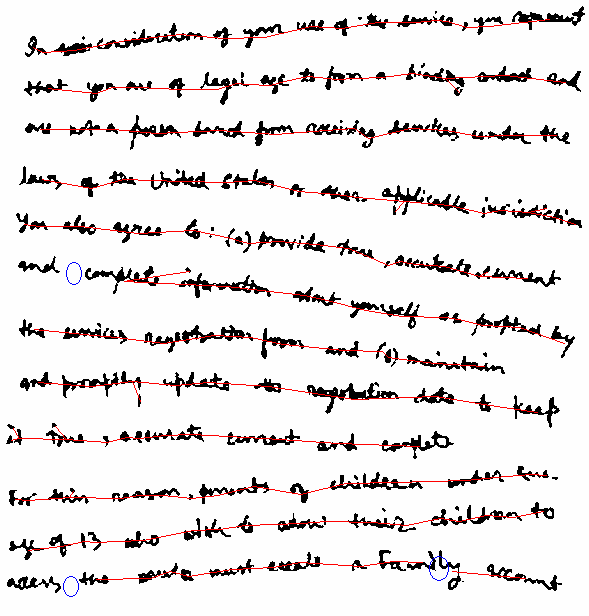
\includegraphics[height=8cm]{images/mst-example-01.png}
    \caption{
        Rezultat pronalaska linija teksta u rukom pisanom dokumentu na
        Engleskom jeziku \citep{yin2007handwritten}
    }
    \label{fig:mst-example-01}
\end{figure}

Motivirani njihovim radom \citep{pan2011hybrid} predstavili su sličan pristup
koji u težinama grafa uzima u obzir dodatne težine koje su učene mjerom MCE
\engl{minimum classification error}.

Još jedan pristup predložili su \citep{DBLP:journals/corr/abs-1301-2628} koji
koriste tehniku hijerahijskog grupiranja koji postupno spaja linije koje dijele
znakove dok god postoje linije koje se mogu spojiti.
\citep{DBLP:journals/corr/TianPHLYT16}

Liang i suradnici \citep{liang1996document} predlažu heuristički algoritam za
određivanje strukture teksta. Algoritam radi horizontalnu projekciju (slika
\ref{fig:histogram-projection}) omeđujućih pravokutnika na jednu ravninu i
pronalazi vrhove i doline u histogramu koji prikazuje frekvencije pojavljivanja
projektiranih pravokntnika. Osim ovog pristupa predložili su još jedan koji
spaja dva znaka u jednu cjelinu ako i samo ako su dva znaka dovoljno blizu da
ih ima smisla spojiti. \citep{gupta2006document} također
koriste razne heuristike prema kojima povezuju susjedne omeđujuće pravokutnike.

\begin{figure}[htb]
    \centering
    \captionsetup{justification=centering,margin=2cm}
    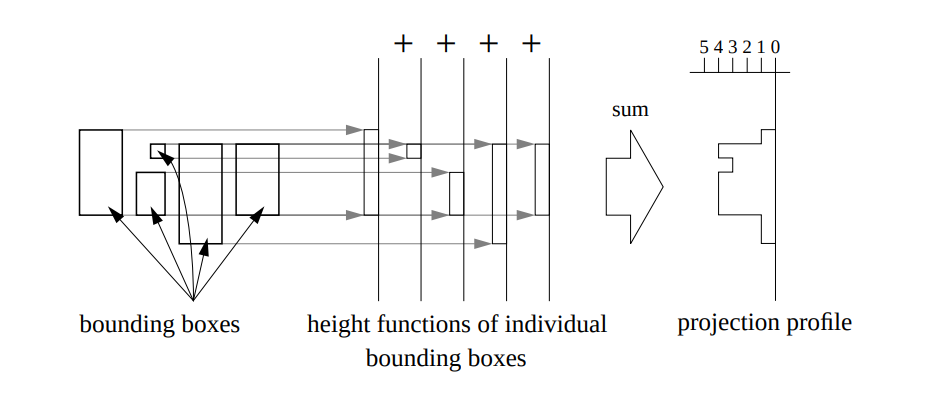
\includegraphics[height=6cm]{images/histogram-projection.png}
    \caption{Histogram dobiven horizontalnom projekcijom omeđujućih pravokutnika \citep{liang1996document}}
    \label{fig:histogram-projection}
\end{figure}

Određivanje strukture teksta je teško i uvelike ovisi o problemu koji
rješavamo. U ovom poglavlju pokazano je da strukturiranje teksta može biti
izvođeno u raznim fazama izvođenja OCR-sustava. Trenutak u kojem ćemo pokrenuti
analizu strukture teksta ovisi o načinu na koji smo označili segmente znakova,
koje informacije o segmentu imamo i koji problem rješavamo. Pokazano je da su
neki pristupi postigli bolje rezultate kada se iskoristilo domensko znanje i
kada su se u nekim heurističkim pristupima koristili parametri koji su bili
pomno izabrani za dani problem. Ovaj rad predložit će nekoliko pristupa za
određivanje strukture teksta na temelju položaja pojedinih znakova nakon
njihove klasifikacije.
















\chapter{Određivanje strukture teksta na temelju položaja pojedinih znakova}
U kontekstu određivanja strukture teksta na temelju položaja pojedinih znakova,
radi preglednije analize, razmatra se OCR-sustav koji nema
korak naknadne obrade. Nakon završetka klasifikacije OCR-sustav posjeduje
nestrukturirani OCR-rezultat u kojem se nalaze svi segmentirani i
klasificirani znakovi. Takav nestrukturirani OCR-rezultat prosljeđuje se
sustavu za određivanje strukture teksta na naknadnu obradu. U praksi je sustav
za određivanje strukture teksta sastavni dio naknadne obrade OCR-sustava,
međutim, u ovaj rad razdvojit će ta dva sustava radi preglednije analize
njihove suradnje koja je prikazana na slici \ref{fig:sustav-01}.

\

\begin{figure}[htb]
    \centering
    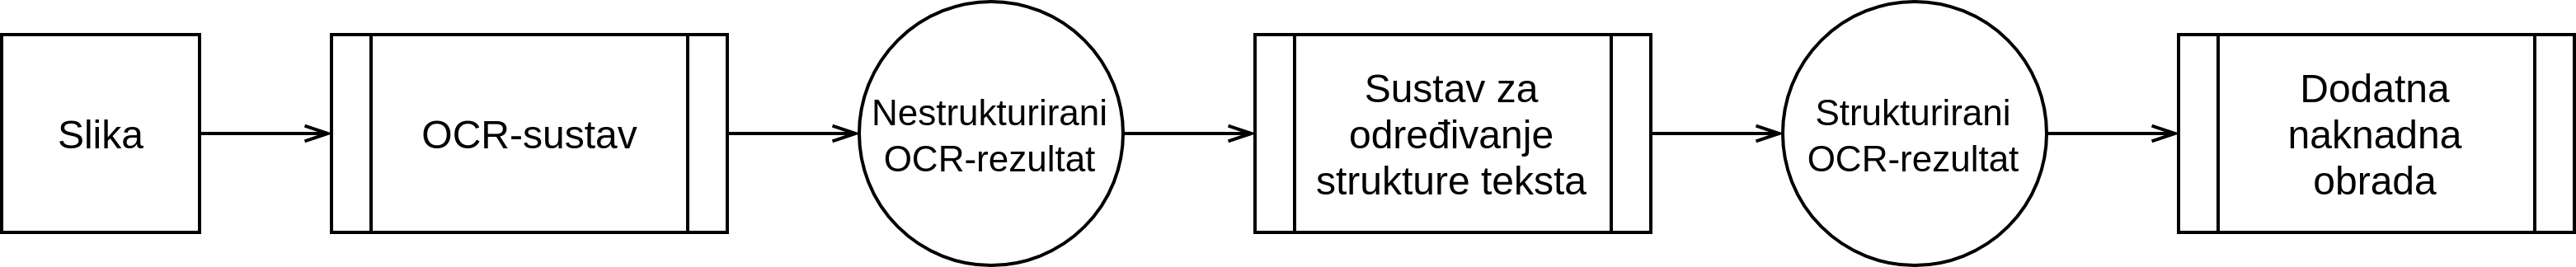
\includegraphics[width=\textwidth]{images/sustav-01.png}
    \caption{Suradnja OCR-sustava i sustava za određivanje strukture teksta.}
    \label{fig:sustav-01}
\end{figure}

Sustav za određivanje strukture teksta na temelju položaja pojedinih znakova
(u daljnjem tekstu: \emph{Sustav}) na ulaz od OCR-sustava prima
nestrukturirani OCR-rezultat koji u sebi sadrži sve znakove koje je OCR-sustav
prepoznao. Svaki znak u OCR-rezultatu posjeduje sljedeće informacije:
\begin{itemize}
    \item[$\bullet$] $x$ - horizontalnu poziciju gornjeg lijevog kuta,
    \item[$\bullet$] $y$ - vertikalnu poziciju gornjeg lijevog kuta,
    \item[$\bullet$] $width$ - širinu znaka,
    \item[$\bullet$] $height$ - visinu znaka i
    \item[$\bullet$] $value$ - Unicode vrijednost znaka.
\end{itemize}

\

Izlaz iz sustava je strukturirani OCR-rezultat u kojemu su znakovi
grupirani u linije, a unutar svake linije riječi su odvojene znakom
bjeline. Strukturirani OCR-rezultat se zatim prosljeđuje dodatnim naknadnim
obradama koje ovise o problemu koji se rješava.

U sklopu ovog rada potrebno je razviti sustav za određivanje strukture
teksta koji će rješavati problem određivanja strukture teksta na računima iz
trgovine i sadržaja iz knjiga. Stup podataka za testiranje
sustava detaljno je objašnjen u odjeljku \ref{sec:skup-padataka-za-testiranje}.

Slika \ref{fig:book-example-02} prikazuje vizualizaciju rezultata OCR-sustava
koji je za svaki znak vratio omeđujući pravokutnik (označeno plavom bojom) i
vrijednost znaka odnosno klasu kojoj znak pripada.
Slike \ref{fig:receipt-example-01} i \ref{fig:book-example-01} također prikazuju
vizualizaciju rezultata OCR-sustava i primjere s kakvim će se sustav susresti.

Primjer pojednostavljenog (detaljnije u odjeljku
\ref{sec:skup-padataka-za-testiranje}) nestrukturiranog OCR-rezultata u formatu
JSON koji će sustav za određivanje strukture teksta dobiti kao svoj ulaz
prikazan je isječkom \ref{lst:ocr-result-json-01}. Ulazni nestrukturirani
OCR-rezultat u formatu JSON uvijek se sastoji od jedne linije u koju
su smješteni svi segmentirani i klasificirani znakovi u nasumičnim redoslijedom.

\

\begin{figure}[htb]
    \centering
    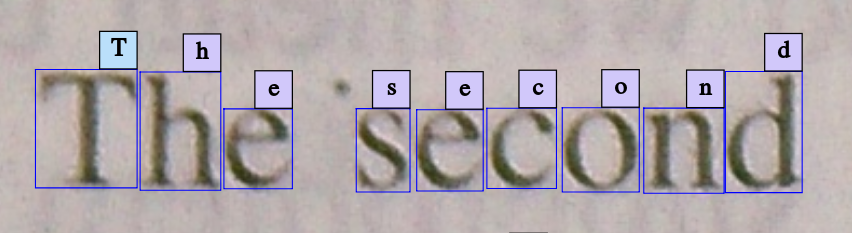
\includegraphics[width=\textwidth]{images/book-example-02.png}
    \caption{Vizualizacija OCR-rezultata.}
    \label{fig:book-example-02}
\end{figure}

\pagebreak

\begin{lstlisting}[
    caption={Pojednostavljeni nestrukturirani OCR-rezultat u formatu JSON.},
    label={lst:ocr-result-json-01},
    firstnumber=1
]
{
    "ocr_result": {
        "lines": [
            {
                "chars": [
                    {
                        "x": 25.95604, "y": 17.30562,
                        "width": 10.64438, "height": 16.60289,
                        "value": 48
                    },
                    {
                        "x": 19.77133, "y": 1.28793,
                        "width": 16.07777, "height": 10.76925,
                        "value": 77
                    },
                    {
                        "x": 5.50248, "y": 2.84320,
                        "width": 12.13375, "height": 15.60966,
                        "value": 73
                    },
                    {
                        "x": 3.19550, "y": 19.67606,
                        "width": 14.94088, "height": 20.78798,
                        "value": 91
                    },

                ]
            }
        ]
    }
}
\end{lstlisting}

\pagebreak








\section{Željena funkcionalnost}
\label{sec:željena-funkcionalnost}
Od sustava se očekuje da za dobiveni nestrukturirani OCR-rezultat u formatu
JSON vrati novi strukturirani OCR-rezultat u istom formatu koji će znakove
grupirati u linije i koji će unutar linija biti poredani s lijeva na desno.
Također, linije moraju biti sortirane tako da se najviša linija u dokumentu
nalazi na prvom mjestu.

Osim grupiranja linija od sustava se očekuje da između dva znaka, gdje smatra da
završava prethodna i započinje nova riječ, ubaci novi znak bjeline čija je
vrijednost \engl{value} $32$, a ostale informacije mogu biti proizvoljne.
Dodatan zahtjev je da sustav sve grupirane linije smjesti u jedan blok
(detaljnije u pododjeljku \ref{subsec:ulazne-datoteke}).

Isječak \ref{lst:ocr-result-json-02} prikazuje primjer izlaza iz sustava za dani
ulaz iz isječka \ref{lst:ocr-result-json-01}. Sustav je znakove grupirao u dvije
linije i između prvog i zadnjeg znaka u drugoj liniji je ubacio znak bjeline.
Vrijednost znaka bjeline je zahtijevana vrijednost $32$. Ostale informacije
znaka bjeline mogle su biti proizvoljne, međutim, sustav im je dodijelio
sljedeće smislenije vrijednosti:\begin{itemize}
    \item[$\bullet$] $x$ - horizontalna pozicija gornjeg desnog kuta lijevog
                           znaka,
    \item[$\bullet$] $y$ - vertikalna pozicija gornjeg lijevog kuta desnog
                           znaka,
    \item[$\bullet$] $width$ - horizontalna udaljenost između gornjeg desnog
                               kuta lijevog znaka i gornjeg lijevog kuta desnog
                               znaka,
    \item[$\bullet$] $height$ - visina lijevog znaka.
\end{itemize}

Pod \emph{lijevi znak} podrazumijeva se na znak koji se nalazi prije znaka
bjeline, a pod \emph{desni znak} podrazumijeva se na znak koji se nalazi nakon
znaka bjeline.

\pagebreak

\begin{lstlisting}[
    caption={Izlaz iz sustava za određivanje strukture teksta u formatu JSON.},
    label={lst:ocr-result-json-02},
    firstnumber=1
]
{
    "ocr_result": {
        "lines": [
            {
                "chars": [
                    {
                        "x": 5.50248, "y": 2.84320,
                        "width": 12.13375, "height": 15.60966,
                        "value": 73
                    },
                    {
                        "x": 19.77133, "y": 1.28793,
                        "width": 16.07777, "height": 10.76925,
                        "value": 77
                    }
                ]
            },
            {
                "chars": [
                    {
                        "x": 3.19550, "y": 19.67606,
                        "width": 14.94088, "height": 20.78798,
                        "value": 91
                    },
                    {
                        "x": 18.13638, "y": 19.67606,
                        "width": 7,81966, "height": 20.78798,
                        "value": 32
                    }
                    {
                        "x": 25.95604, "y": 17.30562,
                        "width": 10.64438, "height": 16.60289,
                        "value": 48
                    }
                ]
            }
        ]
    }
}
\end{lstlisting}








\section{Skup podataka za testiranje}
\label{sec:skup-padataka-za-testiranje}
Skup podataka za testiranje (u daljnjem tekstu: \emph{podatci})
sustava sastoji se od slika, ulaznih datoteka u formatu JSON i
očekivanih izlaznih datoteka. U sklopu ovog rada razvijeni sustav za
određivanje strukture teksta rješavat će problem određivanja strukture teksta
na računima iz trgovine i sadržaja iz knjiga.




\subsection{Slike}
\label{subsec:slike}
Podatci za testiranje sustava sadrže $100$ slika računa (primjer na slici
\ref{fig:receipt-example-04}) i $34$ slike sadržaja iz knjiga (primjer na slici
\ref{fig:book-example-03}).

Svaki znak na svakoj slici je \textbf{ručno} označen i klasificiran. Na slikama
računa iz trgovine označeno je ukupno $85068$ znakova, a na slikama sadržaja iz
knjiga označeno je ukupno $25092$ znaka. Ručno označeni podatci oponašaju
nestrukturirane OCR-rezultate koji su ulaz u sustav za određivanje strukture
teksta.

Omeđujući pravokutnici označenih znakova predstavljaju područje koje označeni
znak zauzima na slici. Stranice omeđujućih pravokutnika su uvijek paralelne sa
rubovima slike. Slika \ref{fig:book-example-04} prikazuje isječak slike,
sadržaja iz knjige, na kojoj su znakovi ukošeni, a stranice njihovih omeđujućih
znakova paralelne su sa rubovima slike. Možemo uočiti kako je moguće da se dva
susjedna omeđujuća pravokutnika preklapaju.

\

\begin{figure}[!htb]
    \centering
    \captionsetup{justification=centering,margin=2cm}
    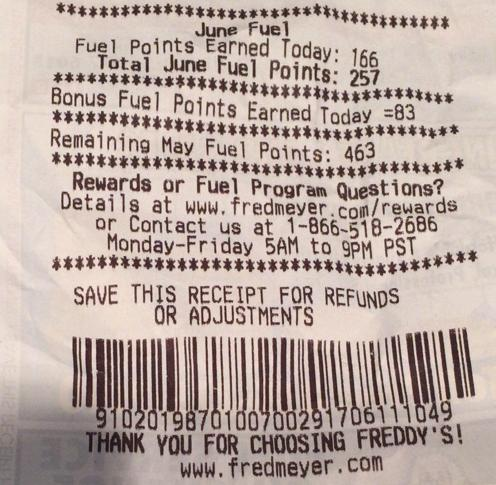
\includegraphics[height=8cm]{images/receipt-example-04.jpg}
    \caption{Primjer slike računa iz trgovine.}
    \label{fig:receipt-example-04}
\end{figure}

\pagebreak

\begin{figure}[htb]
    \centering
    \captionsetup{justification=centering,margin=2cm}
    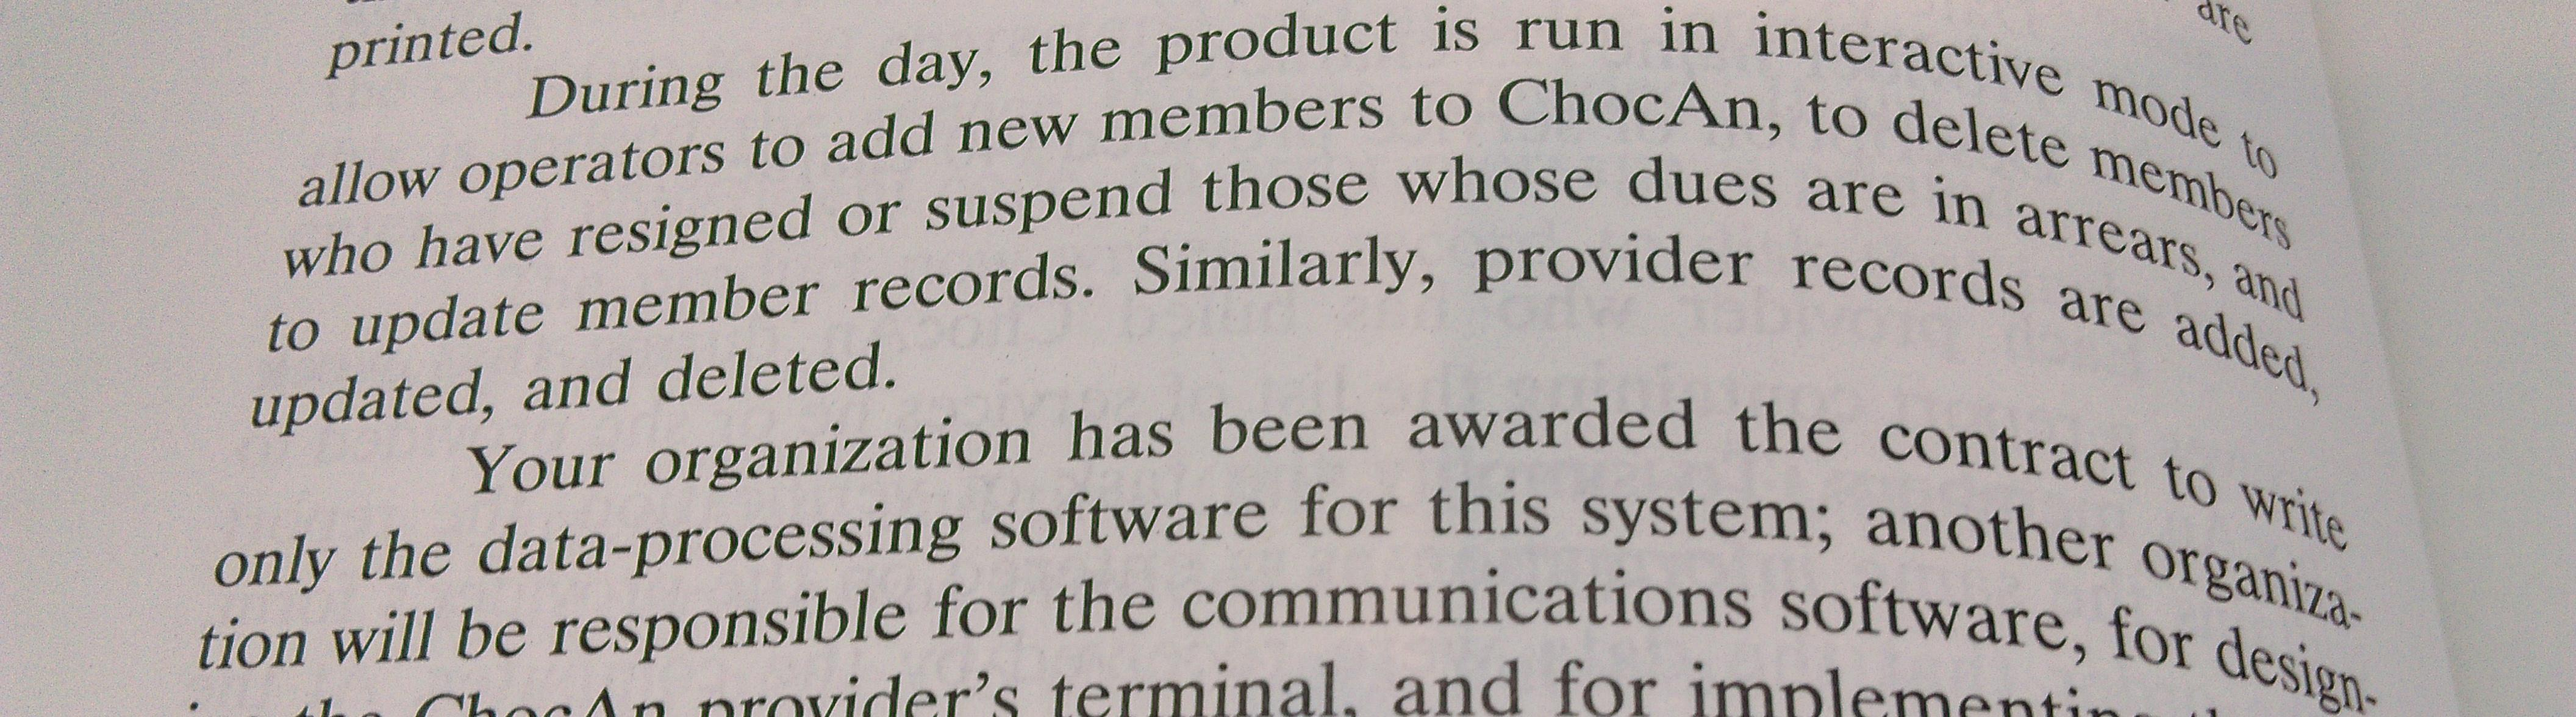
\includegraphics[width=\textwidth]{images/book-example-03.jpg}
    \caption{Primjer slike sadržaja iz knjige.}
    \label{fig:book-example-03}
\end{figure}

\begin{figure}[htb]
    \centering
    \captionsetup{justification=centering,margin=2cm}
    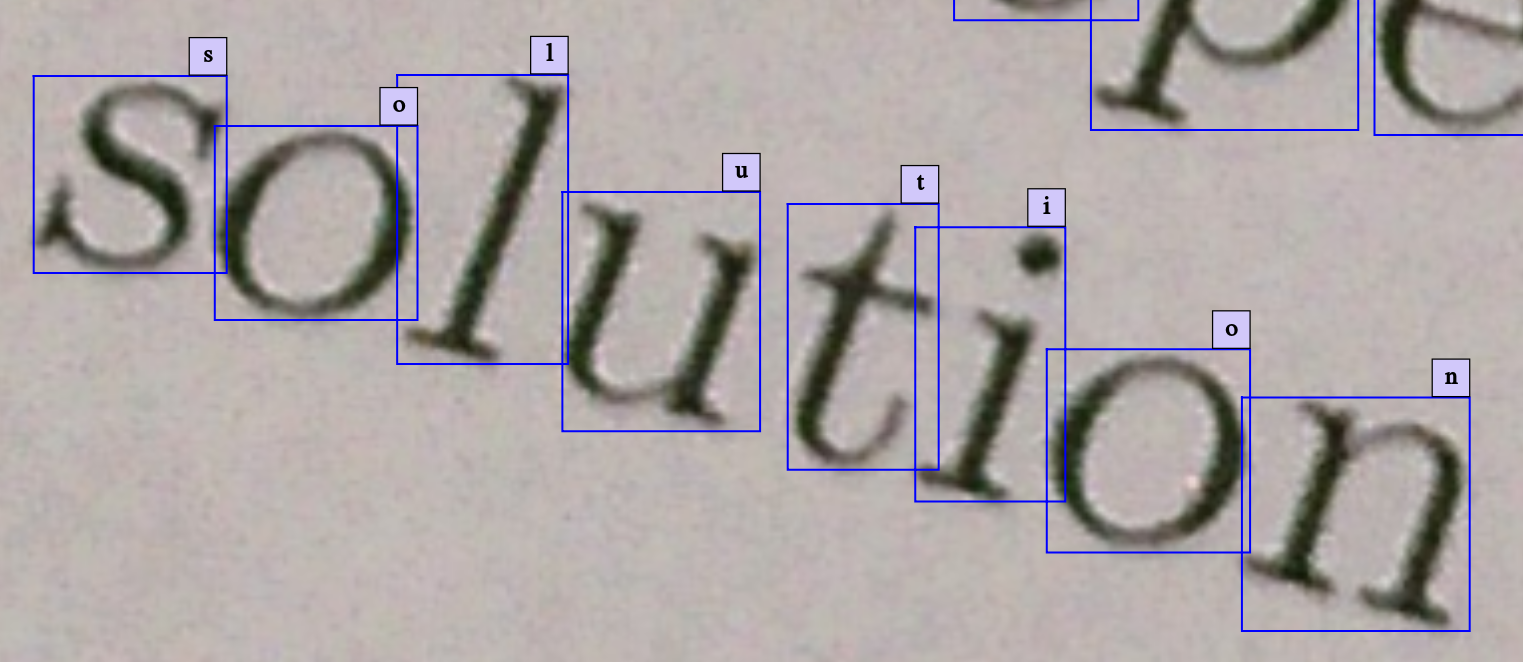
\includegraphics[width=\textwidth]{images/book-example-04.png}
    \caption{Primjer slike s kosim tekstom.}
    \label{fig:book-example-04}
\end{figure}

\pagebreak




\subsection{Ulazne datoteke}
\label{subsec:ulazne-datoteke}
Slike opisane u pododjeljku \ref{subsec:slike} \textbf{ne predstavljaju} ulaz u sustav za određivanje strukture teksta. Nakon označavanja slika podatci o označavanju svake slike se izvoze i pohranjuju u datoteke u formatu JSON. Datoteke u formatu JSON predstavljaju nestrukturirani OCR-rezultat i ulaz u sustav. Ulazna datoteka u formatu JSON u kojoj su zapisani podaci o označavanju slike \ref{fig:receipt-example-04} prikazana je u isječku \ref{lst:ocr-result-json-03}. Zbog specifičnosti sustava za označavanje slika i načina na koji pohranjuje informacije o označavanju, svi označeni znakovi bit će smješteni u jednu liniju u nasumičnom poretku i ta linija će biti smještena u jedan blok. Za svaki znak dostupna je informacija o Unicode vrijednosti znaka koja je smještena pod ključem \lstinline{value}. Dodatno, za svaki znak dostupna je informacija o poziciji i veličini njegovog omeđujućeg pravokutnika \engl{bounding box}. Za svaki omeđujući pravokutnik poznate su sljedeće informacije:

\begin{itemize}
    \item[$\bullet$] $x$ - horizontalna pozicija gornjeg lijevog kuta,
    \item[$\bullet$] $y$ - vertikalna pozicija gornjeg lijevog kuta,
    \item[$\bullet$] $width$ - širina i
    \item[$\bullet$] $height$ - visina.
\end{itemize}

Kako vrijednost $x$ omeđujućeg pravokutnika raste tako je znak bliže desnom rubu
slike i kako vrijednost $y$ omeđujućeg pravokutnika raste tako je znak bliže
donjem rubu slike. Sve informacije o omeđujućem pravokutniku su vrijednosti iz
skupa nenegativnih realnih brojeva.

Sustav za označavanje slika izvozi još neke dodatne informacije o znakovima i
o označenoj slici. Sve informacije koje nisu ovdje navede mogu se zanemariti.

\pagebreak

\begin{lstlisting}[
    caption={
        JSON datoteka s podatcima o označavanju slike
        \ref{fig:receipt-example-04}.
    },
    label={lst:ocr-result-json-03},
    firstnumber=1
]
{
    "ocr_result": {
        "blocks": [
            {
                "lines": [
                    {
                        "chars": [
                            {
                                "value": 83,
                                "bounding_box": {
                                    "x": 4.548218,
                                    "y": 271.68826,
                                    "width": 12.136101,
                                    "height": 22.48648
                                }
                            },
                            {
                                "value": 65,
                                "bounding_box": {
                                    "x": 4.244385,
                                    "y": 247.67685,
                                    "width": 12.59581,
                                    "height": 21.750519
                                }
                            },
                            // ostalih 388 znakova
                        ]
                    }
                ]
            }
        ]
    }
}
\end{lstlisting}


\subsubsection{Izlaz iz sustava za određivanje strukture teksta}
U odjeljku \ref{sec:željena-funkcionalnost} navedene su željene funkcionalnosti
sustava i opisan je pojednostavljeni format izlaza iz sustava. Od sustava se
očekuje da rezultat nakon određivanja strukture teksta prikaže u istom formatu
u kojemu je prikazan ulaz u sustav opisan u ovom odjeljku. Sve grupirane linije
potrebno je smjestiti u jedan blok. Sustav ne treba isporučiti informacije koje
su se mogu zanemariti na ulazu.




\subsection{Očekivane izlazne datoteke}
\label{subsec:ocekivane-izlazne-datoteke}
Očekivane izlazne datoteke predstavljaju ispravni strukturirani tekstualni
sadržaj sa slike. Isječak \ref{lst:txt-result-04} predstavlja ispravni
strukturirani tekstualni sadržaj računa sa slike \ref{fig:receipt-example-04}.
U tekstualnom sadržaju ne postoje bjeline prije početka linije koje
postoje u sadržaju na slici. Osim toga, višestruke bjeline u sadržaju na slici
predstavljene su točno jednom bjelinom u tekstualnom sadržaju u datoteci.

\

\begin{lstlisting}[
    caption={
        Tekstualni sadržaj slike \ref{fig:receipt-example-04}.
    },
    label={lst:txt-result-04},
    firstnumber=1
]
POINTS TO $35 REWARD 8770
BALANCE REWARDS ACCT # *********2463
OPENING BALANCE 20820
EVERYDAY POINTS - RETAIL 410
CLOSING BALANCE 21230
*****************************************
Walgreens 01875
ACCT 7681
SEQUENCE 1875220350
PAYMENT FROM PRIMARY
Get the flu shot that helps provide
a lifesaving vaccine to a child in need
Get a Shot. Give a Shot.® It's that easy
Learn more at the pharmacy.
\end{lstlisting}








\section{Korištenje skupa podataka za testiranje}
\label{sec:koristenje-skupa-podataka-za-testiranje}
Slika \ref{fig:sustav-02} prikazuje postupak dobivanja izlazne datoteke iz
strukturiranog OCR-rezultata kojeg je vratio sustav za određivanje strukture
teksta. Ulaz u sustav je ulazna datoteka u formatu JSON koja predstavlja
nestrukturirani OCR-rezultat kao što je opisano u pododjeljku
\ref{subsec:ulazne-datoteke}.

\

\begin{figure}[htb]
    \centering
    \captionsetup{justification=centering,margin=2cm}
    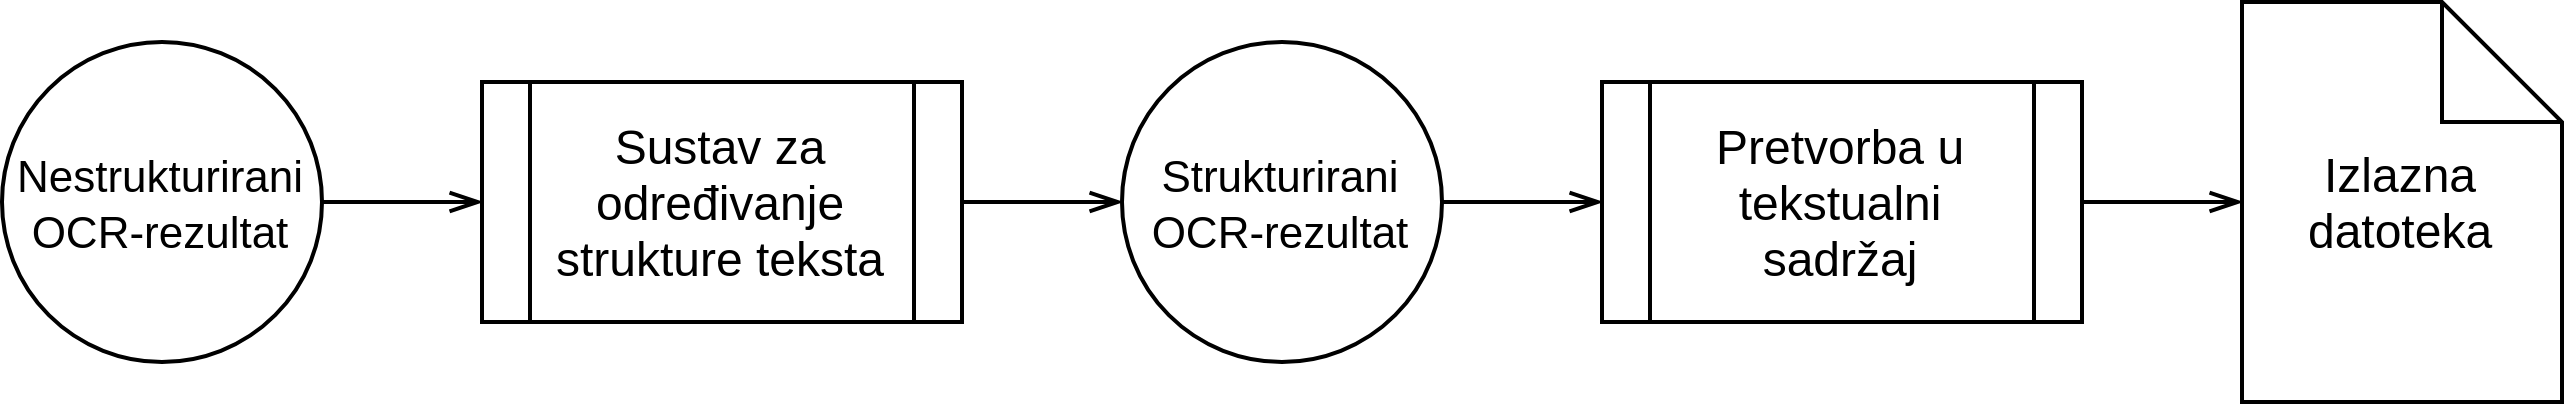
\includegraphics[width=\textwidth]{images/sustav-02.png}
    \caption{
        Postupak dobivanja izlazne datoteke iz strukturiranog OCR-rezultata.
    }
    \label{fig:sustav-02}
\end{figure}

\pagebreak

Izlaz iz sustava je strukturirani OCR-rezultat u
formatu JSON u kojemu se nalaze znakovi grupirani u linije i gdje su između
riječi ubačeni znakovi bjeline. Strukturirani OCR-rezultat potrebno je zapisati
u izlaznu datoteku u formatu opisanom u odjeljku
\ref{subsec:ocekivane-izlazne-datoteke}. Isječak \ref{lst:ocr-result-to-txt}
prikazuje pseudokôd algoritma za ispis OCR-rezultata u format opisan u
pododjeljku \ref{subsec:ocekivane-izlazne-datoteke}. Izlazne datoteke stvorene
na temelju strukturiranih OCR-rezultata i očekivane ulazne datoteke dostupne u
skupu podataka za testiranje uspoređuju se metodom objašnjenom u odjeljku
\ref{sec:mjera-tocnosti-algoritama}.

\

\begin{lstlisting}[
    caption={Pseudokôd algoritma za ispis OCR-rezultata.},
    label={lst:ocr-result-to-txt},
    morekeywords={def,for,end,if,else,return},
    firstnumber=1
]
def ispisi(ocrRezultat)
  for linija u ocrRezultat.linije
    for znak u linija
      print(znak.value)
    end
    print("\n")
  end
end
\end{lstlisting}

















\chapter{Algoritmi za određivanje strukture teksta}
\label{chap:algoritmi-za-odredivanje-strukture-teksta}
Sustav za određivanje strukture teksta podijeljen je u dva podsustava:
\textbf{sustav za određivanje linija} i \textbf{sustav za rastavljanje riječi}.
Slika \ref{fig:sustav-03} prikazuje navedene komponente sustava i njihovu
suradnju. Ulaz u sustav za određivanje linija je nestrukturirani OCR-rezultat
dobiven od OCR-sustava koji je ujedno i ulaz u sustav za određivanje strukture
teksta. Izlaz iz sustava za određivanje linija je OCR-rezultat
u kojemu su znakovi grupirani u linije kojima pripadaju. Izlaz
iz sustava za određivanje linija je ulaz u sustav za rastavljanje riječi koji
u svakoj liniji ubacuje na odgovarajuća mjesta znakove bjeline koji odvajaju
riječi. Izlaz iz sustava za rastavljanje riječi je ujedno i izlaz iz sustava
za određivanje strukture teksta.

\

\begin{figure}[htb]
    \centering
    \captionsetup{justification=centering,margin=2cm}
    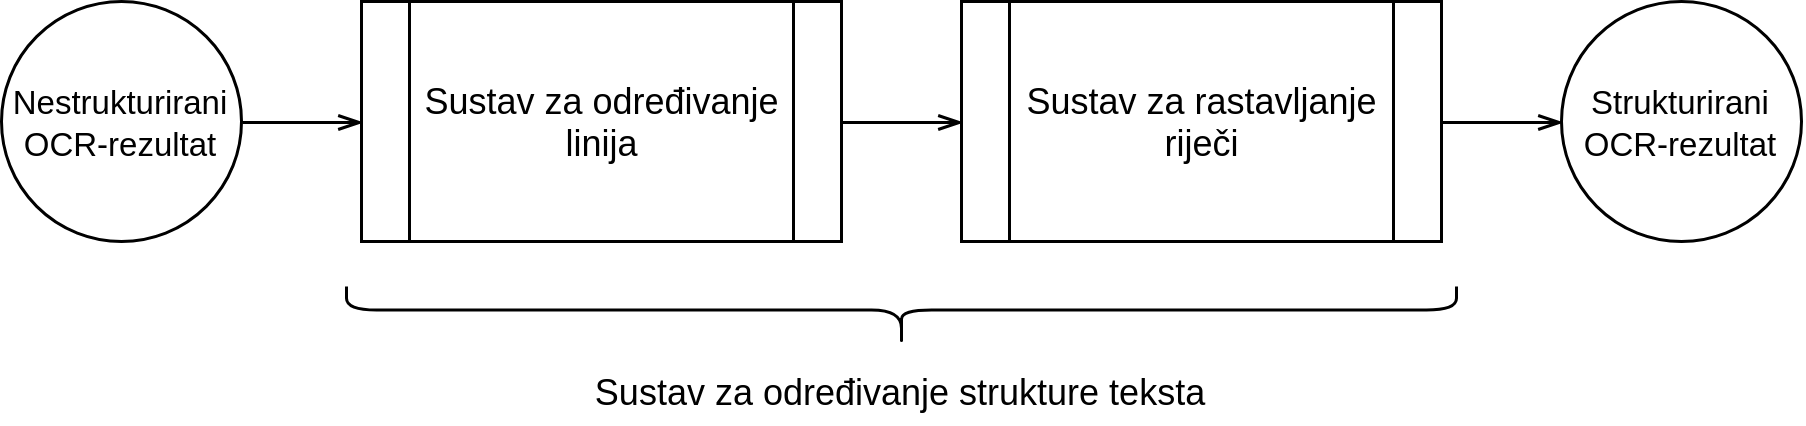
\includegraphics[width=\textwidth]{images/sustav-03.png}
    \caption{
        Komponente sustava za određivanje strukture teksta.
    }
    \label{fig:sustav-03}
\end{figure}

U formalnoj definiciji algoritama koriste se sljedeće oznake:
\begin{itemize}
    \item[$\bullet$] $C$ - označava skup svih znakova u OCR-rezultatu,
    \item[$\bullet$] $A$ i $B$ - označavaju pojedini znak u OCR-rezultatu koji
    ima svoju: širinu $A_w$, visinu $A_h$, horizontalnu poziciju gornjeg
    lijevog kuta $A_x$, vertikalnu poziciju gornjeg lijevog kuta $A_y$ i
    Unicode vrijednost $A_v$,
    \item[$\bullet$] $v$ - označava Unicode vrijednost,
    \item[$\bullet$] $L$ - označava skup svih linija u OCR-rezultatu,
    \item[$\bullet$] $l$ i $k$ - označavaju pojedinu liniju u OCR-rezultatu,
    \item[$\bullet$] $l_{-i}$ - označava $i$-ti znak od kraja linije
    (npr.\ $l_{-1}$ označava zadnji znak u liniji),
    \item[$\bullet$] $l_i$ - označava $i$-ti znak od početka linije (npr.\ $l_1$ označava prvi znak u liniji).
\end{itemize}

\

Linije su skupovi, pa će $|l|$ označavati duljinu linije,
a za znak $A$ reći ćemo da pripada liniji ako vrijedi $A \in l$.
Za dva znaka $A$ i $B$ kažemo da su jednaki ako i samo ako vrijedi:
\[
A = B \iff
A_w = B_w \land A_h = B_h \land A_x = B_x \land A_y = B_y \land A_v = B_v
\]

U definiciji algoritama koristit će se sljedeće horizontalne udaljenosti između dva znaka $A$ i $B$:
\begin{align}
d(A, B) &= |\max(A_x, B_x) - \min(A_x + A_w, B_x + B_w)| \\
d_l(A, B) &= |A_x - B_x| \\
d_c(A, B) &= |A_x + \frac{A_w}{2} - (B_x + \frac{B_w}{2})| \\
\hat{d}(A, B) &= \frac{d(A, B)}{\min(A_w, B_w)} \\
\hat{d_l}(A, B) &= \frac{d_l(A, B)}{\min(A_w, B_w)} \\
\hat{d_c}(A, B) &= \frac{d_c(A, B)}{\min(A_w, B_w)}
\end{align}

Udaljenost $d$ predstavlja udaljenost između desnog ruba lijevog znaka i
lijevog ruba desnog znaka. Udaljenost $d_l$ predstavlja udaljenost lijevih
rubova znakova, a udaljenost $d_c$ predstavlja udaljenost centara znakova.
Udaljenosti $\hat{d}$, $\hat{d_l}$ i $\hat{d_c}$ predstavljaju normalizirane
udaljenosti $d$, $d_l$ i $d_c$.

S ovako definiranim oznakama možemo npr.\ definirati skup svih znakova koji
imaju Unicode vrijednost jednaku $v$:
\[ S(v) = \left\{A \vert A \in C, A_v = v\right\} \]

\pagebreak





\section{Algoritmi za određivanje linija}
\label{sec:algoritmi-za-odredivanje-linija}
Algoritmi za određivanje linija trebaju na temelju omeđujućih pravokutnika
svakog znaka znakove grupirati u linije. Slika \ref{fig:line-semgentation-01}
predstavlja vizualizaciju očekivanog rezultata algoritma za određivanje linija.

\

\begin{figure}[htb]
    \centering
    \captionsetup{justification=centering,margin=2cm}
    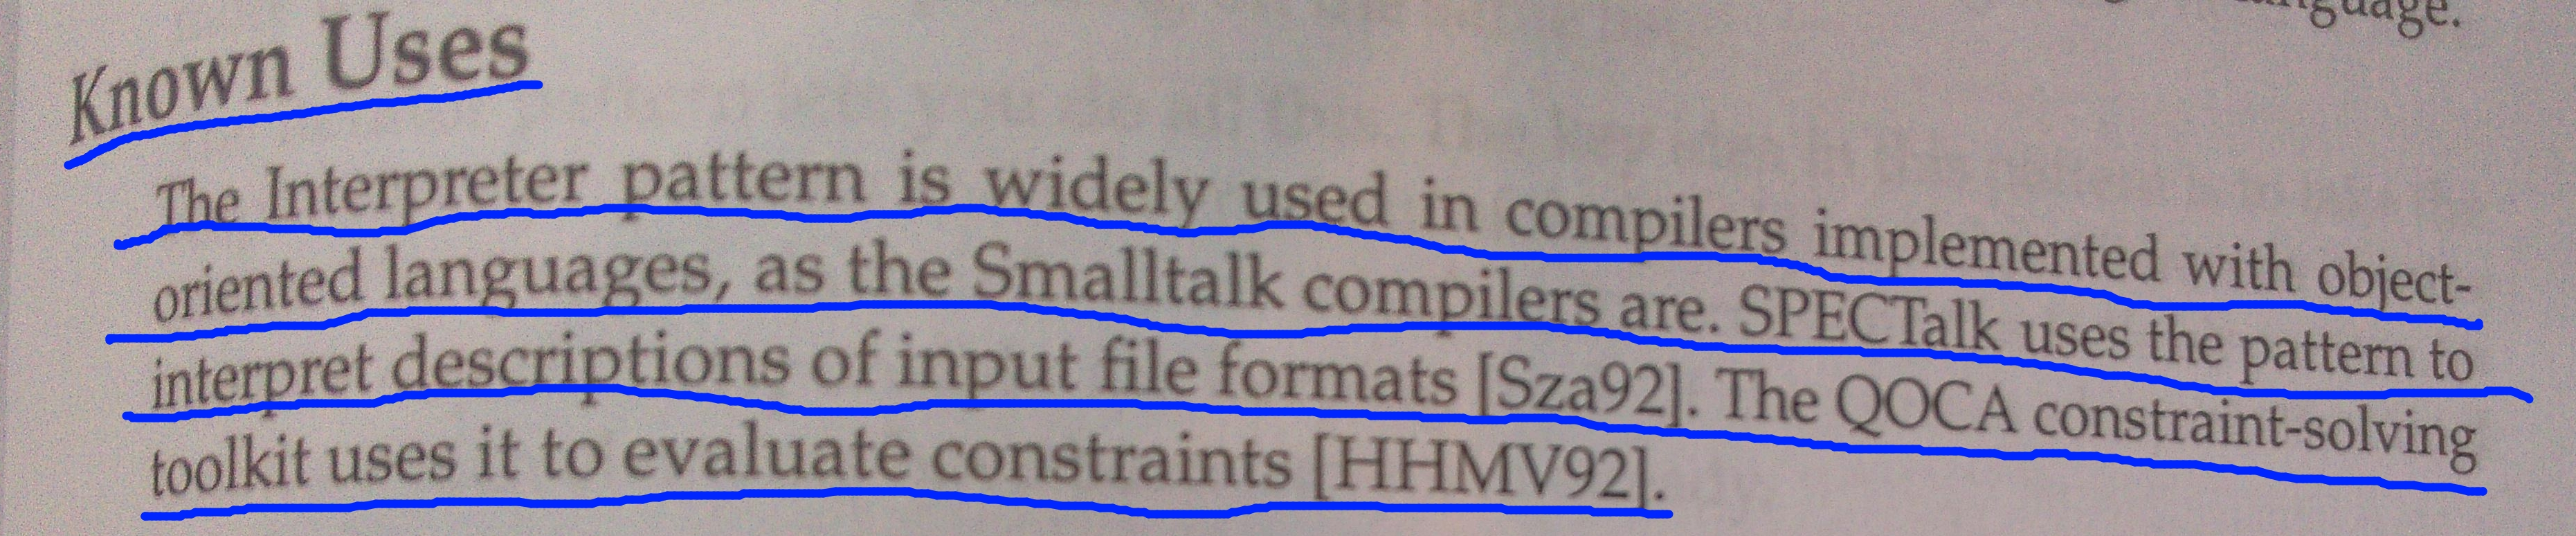
\includegraphics[width=\textwidth]{images/line-segmentation-01.jpg}
    \caption{
        Vizualizacija detektiranih linija u sadržaju iz knjige.
    }
    \label{fig:line-semgentation-01}
\end{figure}

Algoritam na ulazu prima nestrukturirani OCR-rezultat koji je ujedno i ulaz u
sustav za određivanje strukture teksta. Izlaz iz algoritma je OCR-rezultat u
kojemu su znakovi grupirani u linije, sortirani s lijeva na desno i u kojemu
su linije sortirane tako da se najviša linija na slici nalazi na prvom mjestu.

U ovom odjeljku bit će opisan jedan algoritam za određivanje linija temeljen
na maksimalnom preklapanju znakova.



\subsection{Algoritam temeljen na maksimalnom preklapanju znakova}
\label{subsec:algoritam-temeljen-na-maksimalnom-preklapanju-znakova}
Algoritam za određivanje linija temeljen na maksimalnom preklapanja znakova
(u daljnjem tekstu: \emph{algoritam}) temelji se na pretpostavci da dva susjedna
znaka koja se nalaze u istoj liniji ostvaruju maksimalno vertikalno preklapanje.
Vertikalno preklapanje \textit{overlap} dva znaka $A$ i $B$ definira se izrazom:

\begin{equation}
\label{eq:overlap}
\textit{overlap}(A, B) =
\frac{\max(0, \min( A_y + A_h, B_y + B_h ) - \max( A_y, B_y ))}{\min(A_h, B_h)}
\end{equation}

Na početku svog rada algoritam uzlazno sortira sve znakove po horizontalnoj $x$
vrijednost, zatim iterira po svakom znaku i konstruira linije gledajuću s kojom
linijom promatrani znak ostvaruje maksimalno preklapanje. Preklapanje s linijom
definira se kao preklapanje sa zadnjim znakom u toj liniji. Promatrani znak
pripadne onoj liniji s kojom ostvari maksimalno preklapanje:

\begin{equation}
\label{eq:overlap-01}
l_{max} = \argmax_{l \in L}\left\{\textit{overlap}(A, l_{-1})\right\}
\end{equation}

Ako je promatrani znak s nekom linijom ostvario preklapanje vrijednosti $0$
u skup $L$ dodaje se nova linija i promatrani znak postaje početak te linije.
Na ovaj način algoritam konstruira linije i skup svih linija $L$ koji je na
početku prazan.


\subsubsection{Rješavanje problema valovitih linija}
Budući da linije u sadržaju promatranog skupa podataka mogu biti valovite
(slika \ref{fig:aligner-01}), ponekad je poželjno izmjeriti preklapanje ne samo
sa zadnjim znakom u liniji nego i sa zadnjih nekoliko:
\begin{equation}
\label{eq:overlap-02}
l_{max} = \argmax_{l \in L,\ i \in [1, \min(|l|, c_1)]}\left\{\textit{overlap}(A, l_{-i})\right\}
\end{equation}

Za razliku od izraza \ref{eq:overlap-01} koji uzima u obzir samo zadnji znak u
svakoj liniji, izraz \ref{eq:overlap-02} uzet će u obzir zadnjih
$\min(|l|, c_1)$
znakova u svakoj liniji, gdje $c_1$ predstavlja \textbf{parametar algoritma}. Eksperimentalno je utvrđeno da se za vrijednost $1$ parametra $c_1$ ostvaruju najbolji rezultati za sadržaj s računa iz trgovine i da se za vrijednost $2$ parametra $c_1$ ostvaruju najbolji rezultati za sadržaj iz knjiga.

Slika \ref{fig:aligner-01} prikazuje kako znak \lstinline{=} na desnoj strani
crvenog pravokutnika ostvaruje maksimalno preklapanje sa znakom \lstinline{=}
na lijevoj strani crvenog pravokutnika koji nije zadnji znak u liniji u tom
trenutku. Ovakvi i još mnogi drugi primjeri opravdavaju uvođenje parametra
$c_1$.

\begin{figure}[htb]
    \centering
    \captionsetup{justification=centering,margin=2cm}
    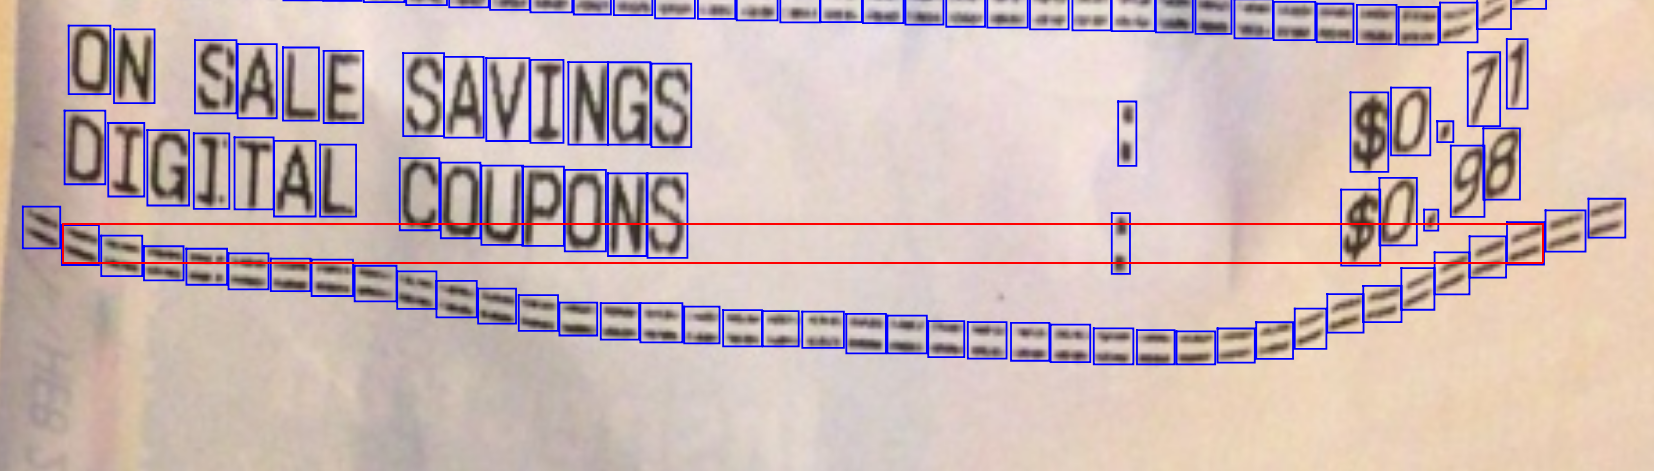
\includegraphics[width=\textwidth]{images/aligner-01.png}
    \caption{Valovite linije otežavaju određivanje linija.}
    \label{fig:aligner-01}
\end{figure}

\pagebreak

\subsubsection{Rješavanje problema preklapanja početaka dviju linija}
Slika \ref{fig:overlap-01} prikazuje kako je moguće preklapanje početaka dviju
linija. Tako znakovi \lstinline{0} i \lstinline{D}
ostvaruju nezanemarivo preklapanje čija će posljedica biti krivo određene
linije. Za uspješno izbjegavanje ovakvih slučajeva uvodi se dodatan uvijet
koji će odlučiti hoće li promatrani znak pripasti liniji s kojom ostvaruje
maksimalno preklapanje:

\begin{equation}
\label{eq:overlap-03}
\max_{i \in [1, \min(|l_{max}|, c_1)]}\left\{\textit{overlap}(A, l_{max_{-i}})\right\} > c_2
\end{equation}

\begin{figure}[htb]
    \centering
    \captionsetup{justification=centering,margin=2cm}
    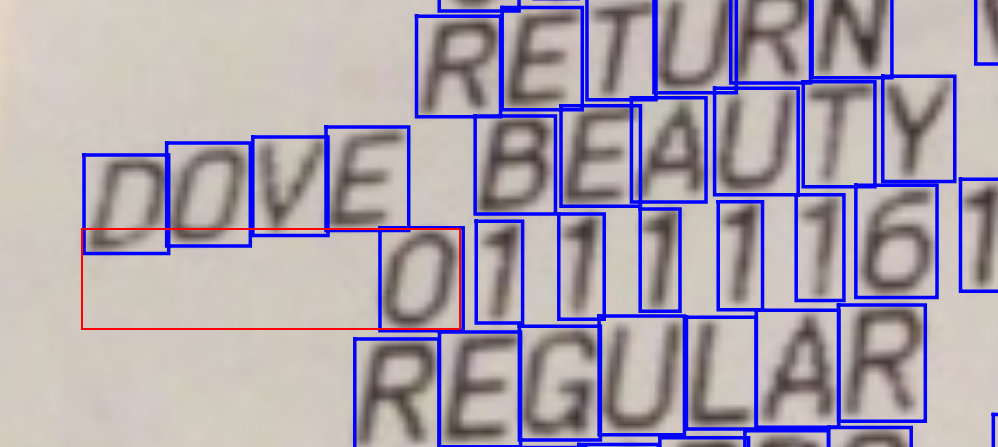
\includegraphics[width=\textwidth]{images/overlap-01.png}
    \caption{Preklapanje početaka dviju linija.}
    \label{fig:overlap-01}
\end{figure}

Nakon što je izrazom \ref{eq:overlap-02} određeno s kojom linijom promatrani
znak ostvaruje maksimalno preklapanje potrebno je provjeriti zadovoljava li iznos
tog preklapanja uvijet naveden izrazom \ref{eq:overlap-03}. Uvodi se novi
parametar algoritma $c_2$ koji predstavlja donju granicu preklapanja koju znak
mora ostvariti s linijom da bi joj se pripojio. Eksperimentalno je utvrđeno da
se za vrijednost $0{,}13$ parametra $c_2$ ostvaruju najbolji rezultati za
sadržaj s računa iz trgovine i da se za vrijednost $0{,}05$ parametra $c_2$
ostvaruju najbolji rezultati za sadržaj iz knjiga.

\begin{figure}[htb]
    \centering
    \captionsetup{justification=centering,margin=2cm}
    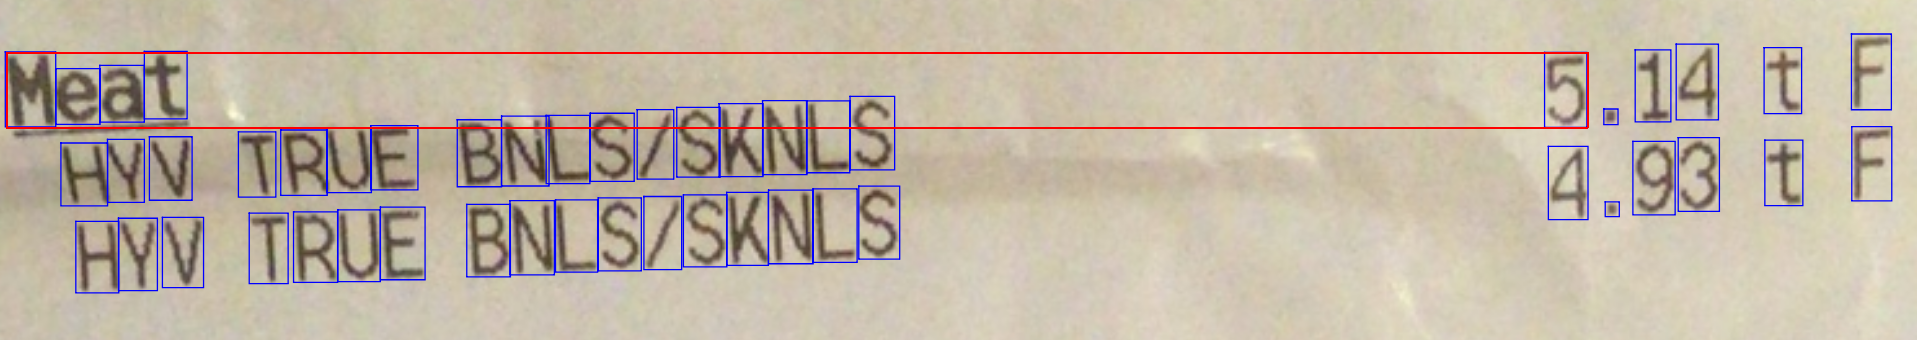
\includegraphics[width=\textwidth]{images/overlap-02.png}
    \caption{Lažno pozitivno preklapanje.}
    \label{fig:overlap-02}
\end{figure}


\subsubsection{Rješavanje problema lažno pozitivnog preklapanja}
Slika \ref{fig:overlap-02} prikazuje slučaj kada znak pripadne krivoj liniji
zato jer s njom ostvaruje maksimalno preklapanje zbog zakrivljenosti slike i
sadržaja. U ovom primjeru znak \lstinline{5} pripast će prvoj liniji
\lstinline{Meat}, a trebao bi pripasti drugoj liniji. Promatrajući skup
podataka za koji se rješava problem zaključeno je kako uvijek treba dati
prednost onoj liniji čiji je zadnji znak bliži znaku kojeg promatramo. Tako će
u primjeru sa slike \ref{fig:overlap-02} znak \lstinline{5} pripasti drugoj
liniji zato jer je njezin zadnji znak bliži znaku \lstinline{5} nego znak
\lstinline{t} iz prve linije i zato jer s zadnjim znakom u drugoj liniji ipak
postiže nezanemarivo preklapanje.

Za rješavanje ovog problema definiraju se dvije funkcije (slika
\ref{fig:function-01})
koje koriste dva nova parametra algoritma $c_3$ i $c_4$:

\begin{align}
f_1(x) &= \frac{1}{1 + c_3 \cdot x} \\[10pt]
f_2(x) &= 1 + \frac{c_4 \cdot x}{1 + c_4 \cdot x}
\end{align}

\begin{figure}[htb]
    \centering
    \captionsetup{justification=centering,margin=2cm}
    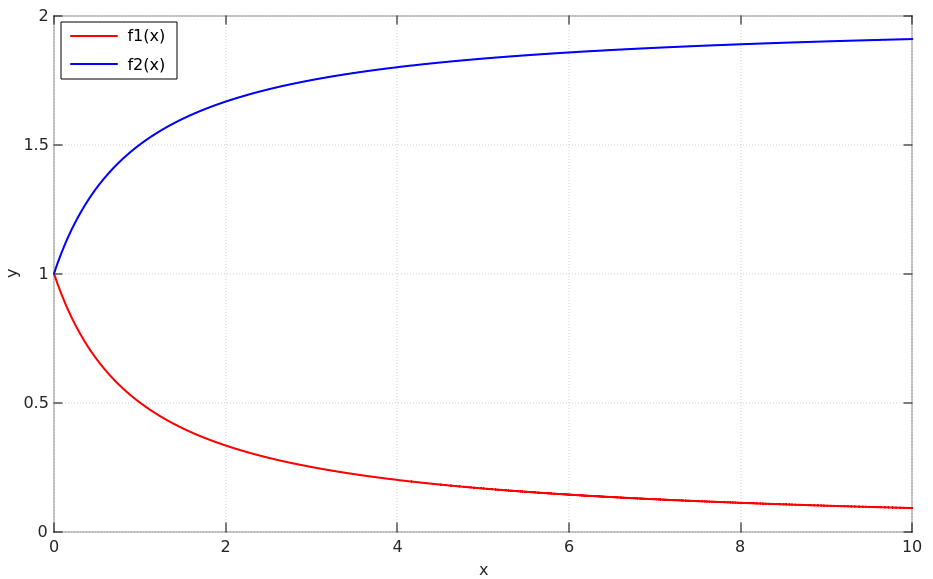
\includegraphics[width=\textwidth]{images/function-01.png}
    \caption{
        Grafovi funkcije $f_1$ (crveno) i funkcije $f_2$ (plavo) za parametre
        $c_3 = c_4 = 1$.
    }
    \label{fig:function-01}
\end{figure}

\pagebreak

Ideja je koristiti navedene funkcije $f_1$ i $f_2$ kako bi se linijama
olakšalo odnosno otežalo postizanje preklapanja u ovisnosti o udaljenosti između
njihovih zadnjih znakova. Recimo da u smo u postupku traženja maksimalnog
preklapanja u jednom trenutku ostvarili maksimalno preklapanje s linijom $l$
iznosa $p_l$. S idućom linijom $k$ izmjerimo preklapanje $p_k$. Da bi linija
$k$ postigla novo maksimalno preklapanje sa promatranim znakom mora vrijediti
$p_k > p_l$. Međutim, recimo da smo uočili da je zadnji znak linije $k$
bliži promatranom znaku nego zadnji znak linije $l$. Koristeći navedenu
opservaciju možemo liniji $k$ olakšati postizanje novog maksimalnog
preklapanja tako da ostvareno preklapanje linije $l$ umanjimo za neki iznos.
Budući da je zadnji znak linije $k$ bliži promatranom znaku novi uvijet koji
linija $k$ mora zadovoljiti da bi ju smatrali novim maksimalnim preklapanjem
glasi:

\begin{equation}
p_k > p_l \cdot f_1(\hat{d_l}(l_{-1},k_{-1}))
\end{equation}

Funkcija $f_1$ će liniji $k$ pomoći tim više što su zadnji znakovi linija
$l$ i $k$ udaljeniji. Da je zadnji znak linije $k$ bio dalje od
promatranog znaka nego zadnji znak linije $l$ onda bismo liniji $k$ trebali
otežati postizanje novog maksimalnog preklapanja čak i ako vrijedi $p_k > p_l$. U tom slučaju novi uvijet za liniju $k$ glasi:

\begin{equation}
    p_k > p_l \cdot f_2(\hat{d_l}(l_{-1},k_{-1}))
\end{equation}

Funkcija $f_2$ će liniji $k$ otežati tim više što su zadnji znakovi linija
$l$ i $k$ udaljeniji. Eksperimentalno je utvrđeno da se za vrijednosti parametra
$c_3 = c_4 = 0{,}13$ ostvaruju najbolji rezultati za sadržaj s računa iz
trgovine i za sadržaj iz knjiga.

Nakon što je svaki znak smješten u odgovarajuću liniju, linije je potrebno
sortirati uzlazno po $y$ vrijednosti prvih znakova linije. Naime, u početnom
koraku sortiranja znakova po $x$ vrijednosti moguće je da prvi znak
u sortiranim znakovima započinje neku liniju u sadržaju koja nije prva u sadržaju. Taj znak će u algoritmu biti detektiran kao početak nove linije koja će se zatim ubaciti u skup svih linija $L$.

Konačno, pseudokôd algoritma za određivanje linija na temelju maksimalnog
preklapanja znakova prikazan je u isječku. U navedenom isječku funkcije $f_1$ i
$f_2$ implicitno koriste vrijednost $0{,}13$ za parametare $c_3$ i $c_4$.
U pseudokôdu funkcija \lstinline{dln} označava funkciju udaljenosti $\hat{d_l}$.

\pagebreak

\begin{lstlisting}[
    caption={Pseudokôd algoritma za određivanje linija.},
    label={lst:algorithm-01},
    morekeywords={def,for,end,if,else,return,new},
    firstnumber=1
]
def odrediLinije(nestrukturiraniOcrRezultat)
  znakovi = sortirajPoX(nestrukturiraniOcrRezultat.sviZnakovi)
  linije = []

  for znak u znakovi
    maxPreklapanje = 0
    linijaSaMaxPreklapanjem = null
    for linija u linije
      p = 0
      tezina = 1
      for i u [0, min(c1, linija.duljina)]
        p = max(p, overlap(znak, linija[-i]))
      end
      if linijaSaMaxPreklapanjem != null
        if linijaSaMaxPreklapanjem[-1].x < linija[-1].x
          tezina = f1(dln(linijaSaMaxPreklapanjem[-1], linija[-1]))
        else
          tezina = f2(dln(linijaSaMaxPreklapanjem[-1], linija[-1]))
        end
      end
      if p > maxPreklapanje * tezina
        maxPreklapanje = p
        linijaSaMaxPreklapanjem = linija
      end
    end

    if maxPreklapanje > c2
      linijaSaMaxPreklapanjem.nadodaj( znak )
    else
      linije.nadodaj([znak])
    end
  end

  sortiraneLinije = sortirajPoY(linije)

  return new OcrRezultat(sortiraneLinije)
end
\end{lstlisting}


\subsubsection{Vremenska složenost algoritma}
U petlji koja počinje linijom $6$ prolazi se kroz sve znakove koji provjeravaju
s kojom linijom ostvaruju maksimalno preklapanje. U najgorem slučaju potrebno je
svaki znak smjestiti u zasebnu liniju što znači da će zadnji ($n$-ti) znak
provjeriti preklapanje sa svakom linijom (odnosno sa svakim znakom jer je svaki
znak u zasebnoj liniji) što daje složenost $\mathcal{O}(n^2)$, gdje je $n$
ukupan broj znakova. Parametar $c_1$ na prvi pogled utječe na složenost, ali
jednostavnom analizom možemo se uvjeriti da to nije slučaj. Pretpostavimo da
parametar $c_1$ postavimo na vrijednost puno veću od ukupnog broja znakova $n$.
Zadnji znak u petlji s početkom linije $6$ treba provjeriti preklapanje sa
svakom linijom. Dodatno, zbog petlje koja počinje linijom $11$ promatrani znak
mora izmjeriti preklapanje sa svakim znakom u liniji što nas opet dovodi do
složenosti $\mathcal{O}(n^2)$. Budući da sortiranja u linijama $2$ i $36$ imaju
složenost $\mathcal{O}(n \cdot \log(n))$ one ne utječu na ukupnu složenost
algoritma.








\section{Algoritmi za rastavljanje riječi}
\label{sec:algoritmi-za-rastavljanje-riječi}
Algoritmi za rastavljanje riječi na ulaz primaju OCR-rezultat u kojemu su
znakovi grupirani u linije u prethodnom koraku opisanom u odjeljku
\ref{sec:algoritmi-za-odredivanje-linija}. Zadaća algoritama za rastavljanje
riječi je da između znakova, za koje smatra da su završetak prethodne odnosno
početak iduće riječi, ubaci znak bjeline čija će vrijednost \engl{value} biti
$32$, a ostale informacije mogu biti proizvoljne.

Ovaj odjeljak opisat će tri algoritma za rastavljanje riječi:
\begin{itemize}
    \item[$\bullet$] algoritam temeljen na prosječnoj širini znaka
    \item[$\bullet$] algoritam temeljen na prosječnoj relativnoj
                     udaljenosti
    \item[$\bullet$] algoritam temeljen na prosječnoj udaljenosti centara
\end{itemize}




\subsection{Algoritam temeljen na prosječnoj širini znaka}
\label{subsec:algoritam-temeljen-na-prosjecnoj-sirini znaka}
Algoritam temeljen na prosječnoj širini znaka (u daljnjem tekstu:
\emph{algoritam}) najjednostavniji je od svih algoritama u ovom odjeljku.
Algoritam se temelji na pretpostavci da je širina razmaka između
riječi proporcionalna sa prosječnom širinom znakova u promatranoj liniji.
Označimo prosječnu širinu znaka u liniji $l$ sa $\overline{w_l}$:

\begin{equation}
\overline{w_l} = \frac{\mathlarger{\sum}\limits_{A \in l} A_w}{|l|}
\end{equation}

Sada možemo postaviti uvijet koji će odlučiti treba li ubaciti bjelinu između
dva znaka $A$ i $B$:

\begin{equation}
\label{eq:condition-01}
d(A, B) > \overline{w_l} \cdot c_1
\end{equation}

Parametar $c_1$ je jedini \textbf{parametar algoritma} za koji je
eksperimentalno utvrđeno da najbolje rezultate za sadržaj na računima iz
trgovine ostvaruje vrijednost $0{,}8$, a najbolje rezultate za sadržaj iz
knjiga ostvaruje vrijednost $0{,}44$. Isječak \ref{lst:algorithm-02} prikazuje
pseudokôd algoritma za rastavljanje riječi temeljenog na prosječnoj širini
znaka.

\begin{lstlisting}[
    caption={
        Pseudokôd algoritma za rastavljanje riječi temeljenog na
        prosječnoj širini znaka.
    },
    label={lst:algorithm-02},
    morekeywords={def,for,end,if,else,return,while,new},
    firstnumber=1
]
def rastaviRijeci(ocrRezultat)
  for linija u ocrRezultat.linije
    prosjecnaSirina = 0
    for znak u linija
      prosjecnaSirina += znak.width
    end
    prosjecnaSirina /= linija.duljina

    i = 0
    j = 1
    while j < linija.duljina
      udaljenost = d(linija[i], linija[j])
      if udaljenost > prosjecnaSirina * c1
        bjelina = new Znak()
        bjelina.value = 32
        bjelina.x = linija[i].x + linija[i].width
        bjelina.y = linija[i].y
        bjelina.width = udaljenost
        bjelina.height = linija[i].height
        linija.ubaciZnakPrijePozicije(j, znak)
        i += 2
        j += 2
      else
        i++
        j++
      end
    end
  end

  return ocrRezultat
end
\end{lstlisting}

\pagebreak

Algoritam prikazan pseudokôdom \ref{lst:algorithm-02} ubacuje znak bjeline
čija je vrijednost jednaka $32$, a ostale informacije su određene na sljedeći
način:
\begin{itemize}
    \item[$\bullet$] $x$ - horizontalna pozicija gornjeg desnog kuta lijevog
                           znaka,
    \item[$\bullet$] $y$ - vertikalna pozicija gornjeg lijevog kuta desnog
                           znaka,
    \item[$\bullet$] $width$ - horizontalna udaljenost između gornjeg desnog
                               kuta lijevog znaka i gornjeg lijevog kuta desnog
                               znaka,
    \item[$\bullet$] $height$ - visina lijevog znaka.
\end{itemize}

Pod \emph{lijevi znak} misli se na znak u liniji na poziciji $i$, a pod
\emph{desni znak} misli se na znak u liniji na poziciji $j$. U liniji $20$
ubacuje se novi znak bjeline prije znaka na poziciji $j$ što
ima za posljedicu pomicanje svih elemenata desno od $j$, uključujući i element
na poziciji $j$, za jedno mjesto udesno.


\subsubsection{Vremenska složenost algoritma}
Ako su u najgorem slučaju svi znakovi smješteni u istu liniju vremenska
složenost ovog algoritma bit će $\mathcal{O}(n)$, gdje je $n$ ukupan broj
znakova. U analizi vremenske složenosti nije uzeta u obzir vremenska složenost
ubacivanja elementa u liniji $20$ zato jer postoje
strukture podataka (npr.\ povezana lista) nad kojima je moguće izvesti operaciju
ubacivanja u konstantnoj složenosti $\mathcal{O}(1)$.

\pagebreak







\subsection{Algoritam temeljen na prosječnoj relativnoj udaljenosti}
\label{subsec:algoritam-temeljen-na-prosjecnoj-relativnoj-udaljenosti}
Algoritam temeljen na prosječnoj relativnoj udaljenosti (u daljnjem tekstu:
\emph{algoritam}) temelji se na pretpostavci da je udaljenost znaka $A$ s
vrijednosti \engl{value} $A_v$ proporcionalna s prosječnom udaljenosti koju svi
znakovi s vrijednosti $A_v$ ostvaruju sa svojim susjedima.

Skup svih susjeda znaka $A$ definiramo kao skup svih znakova $B$ koji su
različiti od $A$, koji se nalaze u istoj liniji kao i $A$, i za koje vrijedi:

\begin{equation}
\hat{d_c}(A, B) < c_1 \texttt{.}
\end{equation}

Skup svih susjeda znaka $A$ označit ćemo s $S(A)$. Parametar $c_1$ prvi je
parametar algoritma za koji je eksperimentalno utvrđeno
da se najbolji rezultati za sadržaj s računa iz trgovina postižu za vrijednost
$4{,}0$ i da se najbolji rezultati za sadržaj iz knjiga postižu za vrijednost
$1{,}5$. Parametar $c_1$ kontrolira koliko najviše dva znaka smiju biti udaljena
da bi se smatrali susjedima.

Skup svih susjeda vrijednosti $v$ definiramo kao uniju svih skupova susjeda
znakova $A$ za koje vrijedi $A_v = v$. Formalno, skup svih susjeda vrijednosti
$v$ definiramo kao:

\begin{equation}
s(v) = \bigcup\limits_{A \in C}\left\{S(A) \vert A_v = v\right\}
\end{equation}

Konačno, prosječnu udaljenost znaka $A$ od susjednih znakova definiramo kao
prosječnu udaljenost koju imaju svi znakovi $B$, za koje vrijedi $A_v = B_v$,
sa svojim susjedima:

\begin{equation}
\label{eq:relative-distance-01}
\overline{d_c}(A) =
\frac{
    \mathlarger{\sum}\limits_{B \in C,\ B_v = A_v}
    \Bigg[
    \mathlarger{\sum}\limits_{D \in S(B)} d_c(B, D)
    \Bigg]
}{|s(A_v)|}
\end{equation}

Budući da funkcija $\overline{d_c}$ ne ovisi o $A$ u izrazu
\ref{eq:relative-distance-01} definiramo ju u ovisnosti o vrijednosti $v$:

\begin{equation}
\label{eq:relative-distance-02}
\overline{d_c}(v) =
\frac{
    \mathlarger{\sum}\limits_{B \in C,\ B_v = v}
    \Bigg[
    \mathlarger{\sum}\limits_{D \in S(B)} d_c(B, D)
    \Bigg]
}{|s(v)|}
\end{equation}

Funkcijom $\overline{d_c}$ dobivamo informaciju kolika je prosječna udaljenost
između znakova $A$, za koje vrijedi $A_v = v$, i njihovih susjeda. Sada možemo
dodatnim uvjetom odrediti postoji li razmak između dva susjedna znaka $A$ i $B$.

Algoritam detektira razmak između znakova $A$ i $B$ ako i samo ako vrijedi:
\begin{equation}
\label{eq:relative-distance-03}
    d_c(A, B) > \overline{d_c}(A_v) \cdot c_2 \quad \lor \quad
    d_c(A, B) > \overline{d_c}(B_v) \cdot c_2 \texttt{.}
\end{equation}

Parametar $c_2$ označava drugi parametar ovog algoritma za koji je
eksperimentalno utvrđeno da se najbolji rezultati za sadržaj s računa iz
trgovina postižu za vrijednost $1{,}2$ i da se najbolji rezultati za sadržaj iz
knjiga postižu za vrijednost $1{,}7$. Parametar $c_2$ kontrolira koliko
minimalno udaljenost između znaka $A$ i $B$ treba biti veća od prosječne
udaljenosti $\overline{d_c}$.

Ovaj algoritam pogodan je za održavanje veze između dva znaka koje bi
algoritam opisan u pododjeljku
\ref{subsec:algoritam-temeljen-na-prosjecnoj-sirini znaka} razdvojio znakom
bjeline zbog krive procjene. Ideja ovog algoritma temelji se na
pretpostavci da su znakovi koji imaju istu vrijednost u prosjeku jednako
udaljeni od znakova s kojima su neposredni susjedi. Ovaj algoritam se u ovoj
inačici može koristiti kao dobar pokazatelj da između neka dva znaka zapravo
ne treba ubaciti znak bjeline iako bi možda neki drugi algoritam opisan u ovom
poglavlju ubacio znak bjeline i time vrlo vjerojatno napravio pogrešku.

Isječak \ref{lst:algorithm-03} prikazuje pseudokôd algoritma temeljenog na
prosječnoj relativnoj udaljenosti znakova. U linijama $2$ i $3$ inicijaliziraju
se mape u kojima će se čuvati informacije u ukupnoj udaljenosti susjednih
znakova i o tome koliko susjednih znakova je uzeto u obzir za svaku Unicode
vrijednost. U liniji $7$ koristi se funkcija $d_c$, a u liniji $8$ funkcija
$\hat{d_c}$. U linijama $23$ i $24$ koriste se navedene mape s kojima se računa
prosječna udaljenost koju Unicode vrijednost ostvaruje sa susjednim znakovima,
zatim se u uvjetu u liniji $25$ detektira razmak. U liniji $33$
ubacuje se novi znak bjeline prije znaka na poziciji $j$ što ima za posljedicu
pomicanje svih elemenata desno od $j$, uključujući i element na poziciji $j$,
za jedno mjesto udesno. Algoritam ostale informacije o znaku bjeline
određuje na isti način kao i algoritam opisan u pododjeljku
\ref{subsec:algoritam-temeljen-na-prosjecnoj-sirini znaka}.

\pagebreak

\begin{lstlisting}[
    caption={
        Pseudokôd algoritma za rastavljanje riječi temeljenog na
        prosječnoj relativnoj udaljenosti.
    },
    label={lst:algorithm-03},
    morekeywords={def,for,end,if,else,return,while,new},
    firstnumber=1
]
def rastaviRijeci(ocrRezultat)
  sumMap = map<unicode value, float>()
  cntMap = map<unicode value, int>()

  for linija u ocrRezultat.linije
    for i = 1; i < linija.duljina; i++
      udaljenost = dc(linija[i], linija[i-1])
      normUdaljenost = ndc(linija[i], linija[i-1])
      if normUdaljenost < c1
        sumMap[linija[i].value] += udaljenost
        cntMap[linija[i].value]++
        sumMap[linija[i-1].value] += udaljenost
        cntMap[linija[i-1].value]++
      end
    end
  end

  for linija u ocrRezultat.linije
    i = 0
    j = 1
    while j < linija.duljina
      udaljenost = dc(linija[i], linija[j])
      avgRelDistI = sumMap[linija[i].value]/cntMap[linja[i].value]
      avgRelDistJ = sumMap[linija[j].value]/cntMap[linja[j].value]
      if udaljenost > avgRelDistI * c2 ||
         udaljenost > avgRelDistJ * c2
        bjelina = new Znak()
        bjelina.value = 32
        bjelina.x = linija[i].x + linija[i].width
        bjelina.y = linija[i].y
        bjelina.width = udaljenost
        bjelina.height = linija[i].height
        linija.ubaciZnakPrijePozicije(j, znak)
        i += 2
        j += 2
      else
        i++
        j++
      end
    end
  end

  return ocrRezultat
end
\end{lstlisting}


\subsubsection{Vremenska složenost algoritma}
Ako su u najgorem slučaju svi znakovi smješteni u istu liniju vremenska
složenost ovog algoritma bit će $\mathcal{O}(n)$, gdje je $n$ ukupan broj
znakova. U analizi vremenske složenosti nije uzeta u obzir vremenska složenost
ubacivanja elementa u liniji $33$ zato jer postoje strukture podataka
(npr.\ povezana lista) nad kojima je moguće izvesti operaciju ubacivanja u
konstantnoj složenosti. U analizi složenosti isto tako nije uzeta u obzir
vremenska složenost ubacivanja i dohvaćanja elemenata iz mape zato jer bismo
takvu mapu mogli ostvariti jednim nizom u kojem bi pozicija ključa bila jednaka
vrijednosti ključa. Korištenje takvog niza omogućilo bi nam da operacije
ubacivanja i dohvaćanja radimo u konstantnom vremenu. Dodatno, korištenje
takvog niza bilo bi memorijski skupo jer bismo u najgorem slučaju trebali imati
mjesta za svaku Unicode vrijednost. Ako bismo htjeli izbjeći takav niz možemo
koristiti mapu s vremenskom složenosti $\mathcal{O}(\log(n))$ za operacije
ubacivanja i dohvaćanja, gdje je $n$ ukupan broj znakova. Korištenjem takve
mape ukupna složenost algoritma bila bi $\mathcal{O}(n \cdot \log(n))$.




\subsection{Algoritam temeljen na prosječnoj udaljenosti centara}
\label{subsec:algoritam-temeljen-na-prosjecnoj-udaljenosti-centara}
Algoritam temeljen na prosječnoj udaljenosti centara (u daljnjem tekstu:
\emph{algoritam}) temelji se na pretpostavci da je širina razmaka između riječi
proporcionalna s prosječnom udaljenosti centara između susjednih znakova.
Skup svih susjeda znaka $A$ definira se na isti način kao i u algoritmu
opisanom u odjeljku
\ref{subsec:algoritam-temeljen-na-prosjecnoj-relativnoj-udaljenosti}. Skup svih
susjeda znaka $A$ definiramo kao skup svih znakova $B$ koji su različiti od $A$,
koji se nalaze u istoj liniji kao i $A$, i za koje vrijedi izraz:

\begin{equation}
\hat{d_c}(A, B) < c_1 \texttt{.}
\end{equation}

Skup svih susjeda znaka $A$ označit ćemo s $S(A)$. Parametar $c_1$ prvi je
parametar algoritma za koji je eksperimentalno utvrđeno
da se najbolji rezultati za sadržaj s računa iz trgovina postižu za vrijednost
$3{,}0$ i da se najbolji rezultati za sadržaj iz knjiga postižu za vrijednost
$1{,}5$. Parametar $c_1$ kontrolira koliko najviše dva znaka smiju biti udaljena
da bi se smatrali susjedima.

\pagebreak

Pomoću skupa $S(A)$ definirat ćemo prosječnu udaljenost centara između
susjednih znakova u liniji $l$:

\begin{equation}
\overline{d_c}(l) =
\frac{
    \mathlarger{\sum}\limits_{A \in l}
    \Bigg[
    \mathlarger{\sum}\limits_{B \in S(A)} d_c(A, B)
    \Bigg]
}
{\bigg|\bigcup\limits_{A \in l} S(A)\bigg|}
\end{equation}

Napokon, algoritam ubacuje znak bjeline između znakova $A$ i $B$ ako je ispunjen
uvijet:

\begin{equation}
d_c(A, B) > \overline{d_c}(l) \cdot c_2 \texttt{.}
\end{equation}

Parametar algoritma $c_2$ kontrolira koliko minimalno udaljenost između znaka
$A$ i $B$ treba biti veća od prosječne udaljenosti centara između susjednih
znakova u liniji $l$ da bi znakovi bili razdvojeni. Eksperimentalno je utvrđeno
da se najbolji rezultati za sadržaj s računa iz trgovina postižu za vrijednost
$1{,}2$ i da se najbolji rezultati za sadržaj iz knjiga postižu za vrijednost
$1{,}4$.

Isječak \ref{lst:algorithm-04} prikazuje pseudokôd algoritma temeljenog na
prosječnoj udaljenosti centara. U liniji $5$ koristi se funkcija $\hat{d_c}$,
a u liniji $6$ funkcija $d_c$. U liniji $24$ ubacuje se novi znak bjeline prije
znaka na poziciji $j$ što ima za posljedicu pomicanje svih elemenata desno od
$j$, uključujući i element na poziciji $j$, za jedno mjesto udesno. Algoritam
ostale informacije o znaku bjeline određuje na isti način kao i algoritam
opisan u pododjeljku
\ref{subsec:algoritam-temeljen-na-prosjecnoj-sirini znaka}.

\pagebreak

\begin{lstlisting}[
    caption={
        Pseudokôd algoritma za rastavljanje riječi temeljenog na
        prosječnoj udaljenosti centara.
    },
    label={lst:algorithm-04},
    morekeywords={def,for,end,if,else,return,while,new},
    firstnumber=1
]
def rastaviRijeci(ocrRezultat)
  for linija u ocrRezultat.linije
    brojac = 0
    for i = 1; i < linija.duljina; i++
      if ndc(linija[i], linija[i-1] < c1
        avgUdaljenost += dc(linija[i], linija[i-1])
        brojac++
      end
    end

    avgUdaljenost /= brojac

    i = 0
    j = 1
    while j < linija.duljina
      udaljenost = dc(linija[i], linija[j])
      if udaljenost > avgUdaljenost * c2
        bjelina = new Znak()
        bjelina.value = 32
        bjelina.x = linija[i].x + linija[i].width
        bjelina.y = linija[i].y
        bjelina.width = udaljenost
        bjelina.height = linija[i].height
        linija.ubaciZnakPrijePozicije(j, znak)
        i += 2
        j += 2
      else
        i++
        j++
      end
    end
  end

  return ocrRezultat
end
\end{lstlisting}


\subsubsection{Vremenska složenost algoritma}
Vremenska složenost algoritma za najgori slučaj je $\mathcal{O}(n)$ budući
da će se svaki znak posjetiti samo jednom. U analizi vremenske složenosti
nije uzeta u obzir vremenska složenost ubacivanja elementa u liniji $24$ zato
jer postoje strukture podataka (npr.\ povezana lista) nad kojima je moguće
izvesti operaciju ubacivanja u konstantnoj složenosti.
















\chapter{Rezultati i analiza}
Ovo poglavlje prikazuje i analizira rezultate rada svakog algoritma
opisanog u poglavlju \ref{chap:algoritmi-za-odredivanje-strukture-teksta}.
U odjeljku \ref{sec:mjera-tocnosti-algoritama} opisana je metoda
za određivanje točnosti svakog algoritma. U odjeljcima
\ref{sec:rezultati-i-analiza-algoritama-za-odredivanje-linija} i
\ref{sec:rezultati-i-analiza-algoritama-za-rastavljanje-rijeci}
prikazani su i analizirani rezultati rada algoritama za određivanje linija i
algoritama za rastavljanje riječi.








\section{Mjere točnosti algoritama}
\label{sec:mjera-tocnosti-algoritama}
U odjeljku \ref{sec:koristenje-skupa-podataka-za-testiranje} opisan je način
uporabe skupa podataka za testiranje. Sustav za određivanje strukture teksta
(u daljnjem tekstu: \emph{Sustav}) na ulaz dobiva nestrukturirani OCR-rezultat,
a na izlazu daje strukturirani OCR-rezultat koji je potrebno zapisati u izlaznu
datoteku u formatu opisanom u pododjeljku
\ref{subsec:ocekivane-izlazne-datoteke}. Sadržaj izlazne datoteke uspoređuje se
sa sadržajem očekivane izlazne datoteke dostupne u skupu podataka za
testiranje. Rezultat usporedbe odredit će točnost sustava za određivanje
strukture teksta.

Za usporedbu sadržaja koristi se Levenshteinova udaljenost između niza znakova
sadržaja očekivane izlazne datoteke i niza znakova sadržaja izlazne datoteke
stvorene na temelju OCR-rezultata dobivenog iz sustava.
Algoritam Levenshteinove udaljenosti dobro je opisan u literaturi i ovaj rad
neće ulaziti u detalje njegova rada.

\begin{lstlisting}[
    caption={Primjer sadržaja očekivane izlazne datoteke.},
    label={lst:output-01},
    firstnumber=1
]
Lorem ipsum dolor sit amet,
consectetur adipiscing elit.
\end{lstlisting}

Način određivanja točnosti pokazat će se na primjeru isječaka
\ref{lst:output-01} i \ref{lst:output-02}. Isječak \ref{lst:output-01}
prikazuje sadržaj očekivane izlazne datoteke, a isječak \ref{lst:output-02}
prikazuje sadržaj izlazne datoteke stvorene na temelju OCR-rezultata dobivenog
iz sustava.

\begin{lstlisting}[
    caption={
        Primjer sadržaja izlazne datoteke stvorene na temelju OCR-rezultata
        dobivenog iz sustava.
    },
    label={lst:output-02},
    firstnumber=1
]
Lorem dolors it amet ,
consecte tur ipsum ad ipiscing elit.
\end{lstlisting}

Sustav je progriješio u određivanju linija time što je riječ \lstinline{ipsum}
stavio u drugu liniju. Osim toga, progriješio je i u razdvajanju riječi u obje
linije. Levenshteinova udaljenost sadržaja te dvije datoteke je $17$, međutim,
ta informacija ne govori ništa o točnosti sustava. Rezultat Levenshteinove
udaljenosti određuje broj pogrešaka koje sustav radi u odnosu na referentne
vrijednosti (očekivane izlazne datoteke). Maksimalan broj pogrešaka koje je
sustav mogao napraviti je zapravo maksimalna moguća Levenshteinova udaljenost
između dva niza znakova, koja je jednaka duljini duljeg niza znakova. U
primjeru, dulji niz znakova je niz znakova iz isječka
\ref{lst:output-02} koji se sastoji od $59$ znakova (uključujući i znak za novi
redak \lstinline{\n}). Sustav je napravio $17$ pogrešaka od maksimalno $59$,
odnosno njegova greška iznosi $\frac{17}{59} \cdot 100\% = 29\%$. Iz pogreške
se može izračunati točnost koja iznosi $71\%$.

Formalno, točnost ili dobrota \engl{fitness} sustava određuje se izrazom:

\begin{equation}
\label{eq:fitness}
f(a, b) = 1 - \frac{d_\textit{levenshtein}(a, b)}{\max(|a|, |b|)} \texttt{.}
\end{equation}

U izrazu su s $a$ i $b$ označeni nizovi znakova, a s
$d_\textit{levenshtein}$ Levenshteinova funkcija udaljenosti. U nastavku ovog
poglavlja točnost sustava iskazivat će se u vrijednostima
između $0$ i $1$, a ne u postocima.

Slika \ref{fig:result-example-01} prikazuje graf točnosti (dobrote) sustava za
određivanje strukture teksta za sadržaj računa iz trgovine. Za svaki testni
primjer izmjerena je dobrota sustava, zatim su izmjerete dobrote uzlazno
sortirane i tako su nanesene na graf dobrote te je zbog toga graf monotono
rastući. Na ovaj će se način prikazivati grafove dobrote u rezultatima svih
algoritama.

\begin{figure}[htb]
    \centering
    \captionsetup{justification=centering,margin=2cm}
    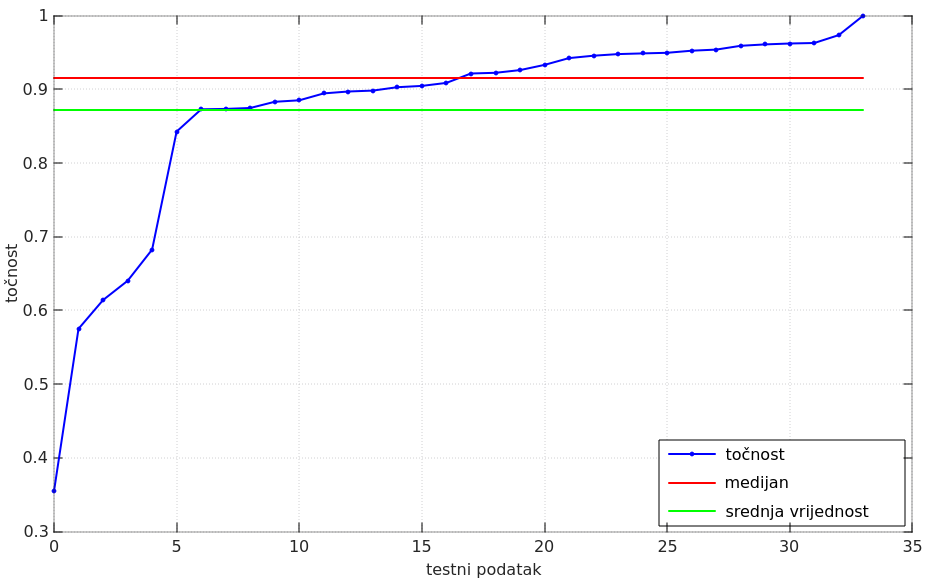
\includegraphics[width=\textwidth]{images/result-example-01.png}
    \caption{Graf točnosti sustava.}
    \label{fig:result-example-01}
\end{figure}

\pagebreak




\subsection{Mjera točnosti algoritama za određivanje linija}
Mjera točnosti algoritama za određivanje linija svodi se na usporedbu
sadržaja očekivane izlazne datoteke iz koje su izbrisani svi znakovi bjeline.
Sadržaj takve (modificirane) datoteke smatra se referentnim sadržajem prilikom
određivanja točnosti. Isječak \ref{lst:output-03} prikazuje referentni sadržaj,
za određivanje točnosti algoritama za određivanje linija, dobiven brisanjem
znakova bjeline iz sadržaja datoteke prikazane isječkom \ref{lst:output-01}.

\begin{lstlisting}[
    caption={
        Primjer referentnog sadržaja datoteke.
    },
    label={lst:output-03},
    firstnumber=1
]
Loremipsumdolorsitamet,
consecteturadipiscingelit.
\end{lstlisting}

Slika \ref{fig:sustav-04} prikazuje postupak dobivanja izlazne datoteke iz
OCR-rezultata s grupiranim linijama. Format izlazne datoteke opisan je u
pododjeljku \ref{subsec:ocekivane-izlazne-datoteke}. Sadržaj dobivene izlazne
datoteke uspoređuje se sa referentnim sadržajem koristeći izraz
\ref{eq:fitness}.

\begin{figure}[htb]
    \centering
    \captionsetup{justification=centering,margin=2cm}
    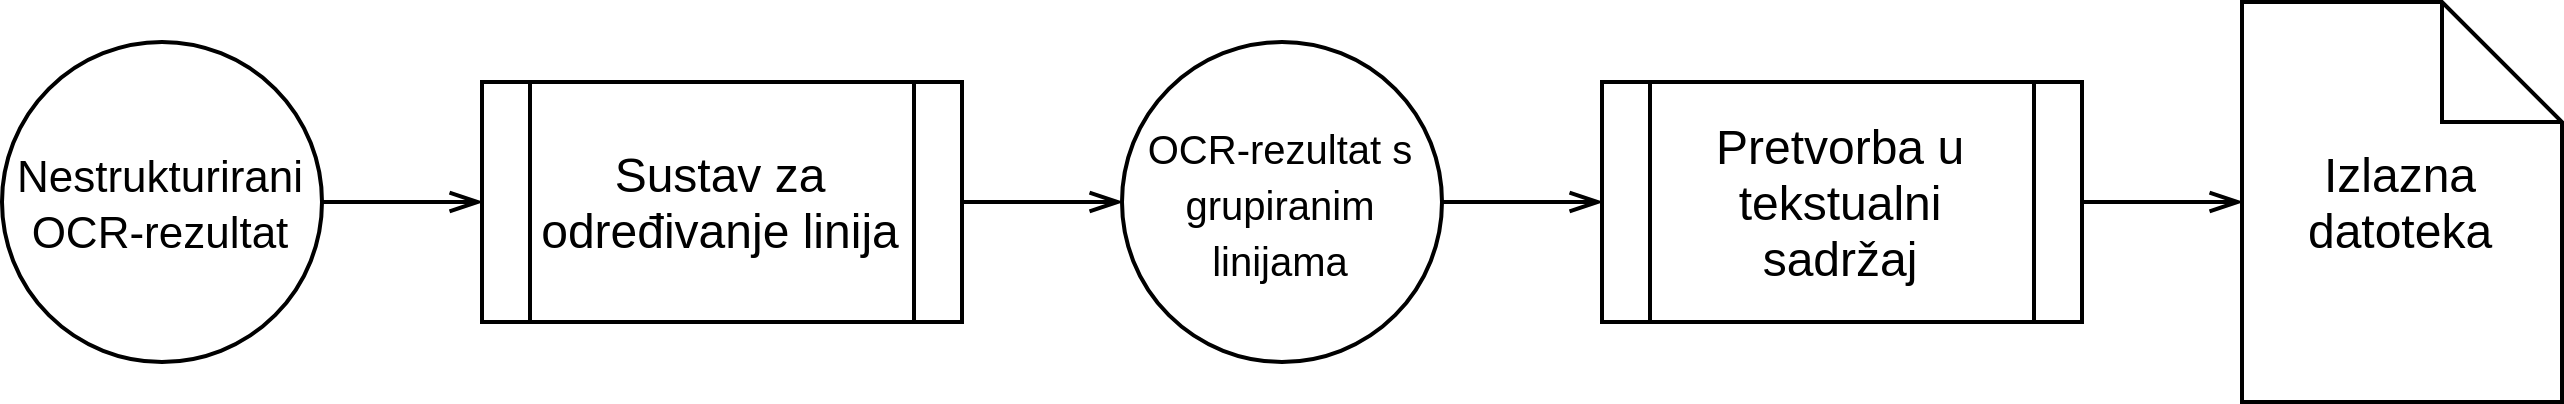
\includegraphics[width=\textwidth]{images/sustav-04.png}
    \caption{
        Postupak dobivanja izlazne datoteke iz OCR-rezultata dobivenog od
        sustava za određivanje linija.
    }
    \label{fig:sustav-04}
\end{figure}

\pagebreak

Isječak \ref{lst:output-04} prikazuje primjer sadržaja izlazne datoteke stvorene
na temelju OCR-rezultata dobivenog od sustava za određivanje linija. U sadržaju
ne postoje razmaci zato jer OCR-rezultat nije još prošao kroz
sustav za rastavljanje riječi. Točnost sadržaja izlazne datoteke u odnosu na
referentni sadržaj iz isječka \ref{lst:output-03} iznosi $0{,}8$.

\begin{lstlisting}[
    caption={
        Primjer sadržaja izlazne datoteke.
    },
    label={lst:output-04},
    firstnumber=1
]
Loremdolorsitamet,
consecteturipsumadipiscingelit.
\end{lstlisting}

Na opisani način računat će se točnost za algoritme za određivanje linija, a
funkcija točnosti prikazivat će se kao na slici \ref{fig:result-example-01}.




\subsection{Mjera točnosti algoritama za rastavljanje riječi}
Za određivanje točnosti algoritama za rastavljanje riječi koriste se, kao
referentne datoteke, očekivane izlazne datoteke koje će se uspoređivati sa
sadržajem izlazne datoteke stvorene na temelju OCR-rezultata dobivenog od
sustava za rastavljanje riječi. Slika \ref{fig:sustav-05} prikazuje postupak
dobivanja izlazne datoteke iz OCR-rezultata dobivenog od sustava za
rastavljanje riječi. Ulaz u sustav za rastavljanje riječi je OCR-rezultat, s
grupiranim linijama, dobiven iz sustava za određivanje linija. Budući da sustav
za određivanje linija ponekad neispravno određuje linije, ne može se od sustava
za rastavljanje riječi očekivati bolja dobrota od dobrote sustava za
određivanje linija. Određivanje točnosti algoritama za rastavljanje riječi je
time ovisno o točnosti algoritama za određivanje linija, što je najveći
nedostatak ovog pristupa za mjerenje točnosti.

Budući da je ulazni OCR-rezultat u sustava za rastavljanje riječi rezultat
kojeg je vratio sustav za određivanje linija, mjera točnosti sustava za
rastavljanje riječi je ujedno i mjera točnosti cijelog sustava za određivanje
strukture teksta zato.

\begin{figure}[htb]
    \centering
    \captionsetup{justification=centering,margin=2cm}
    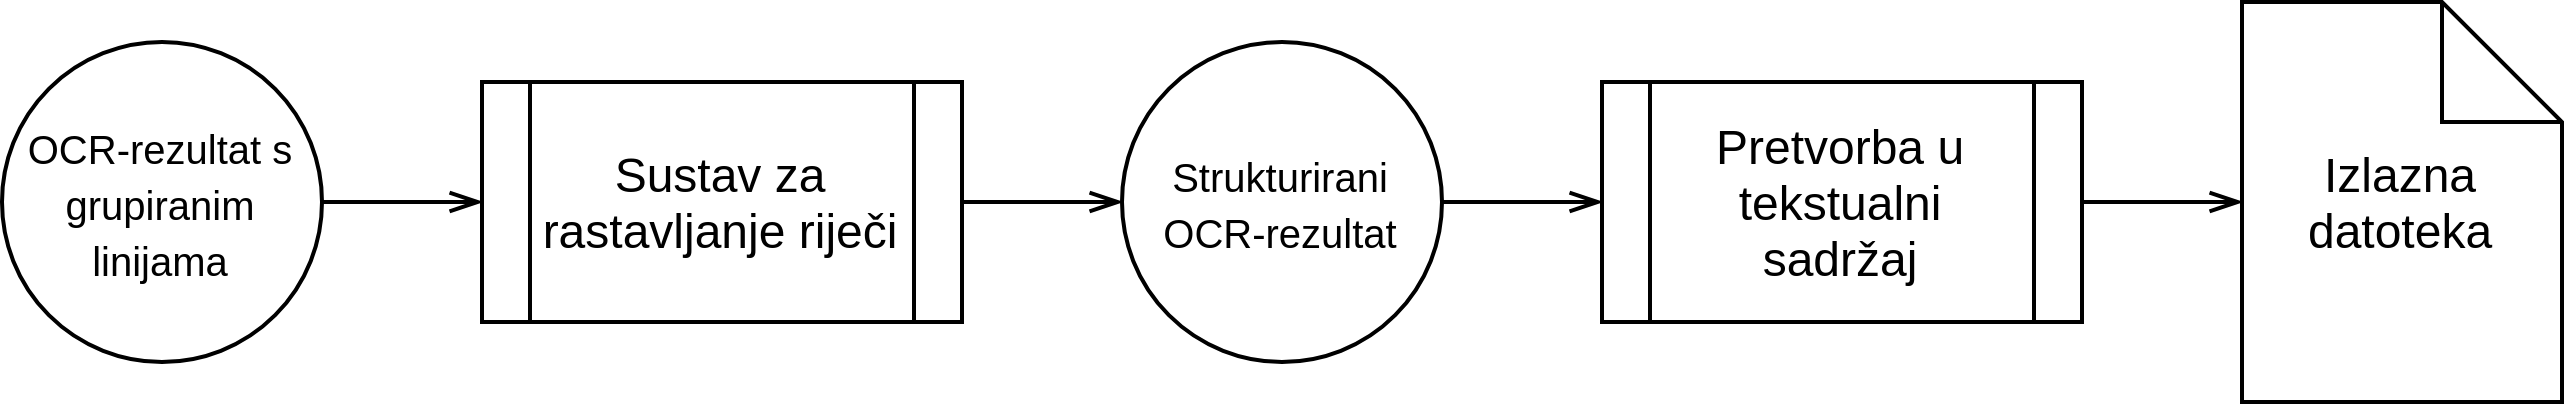
\includegraphics[width=\textwidth]{images/sustav-05.png}
    \caption{
        Postupak dobivanja izlazne datoteke iz OCR-rezultata dobivenog od
        sustava za rastavljanje riječi.
    }
    \label{fig:sustav-05}
\end{figure}

\subsection{Daljnja poboljšanja u određivanju točnosti}
Prednost korištenog skupa za testiranje i opisanih metoda za određivanje
točnosti je to što se lako može generirati veći skup podataka za testiranje
koristeći metodu početnog podizanja \engl{bootstrapping}. Kada su na
raspolaganju samo označeni znakovi s omeđujućim pravokutnicima moguće je, na
temelju nekoliko jednostavnih unaprijed ručno napisanih očekivanih izlaznih
datoteka, napraviti prvu verziju sustava za određivanje strukture teksta.
Analizom rezultata, sustav se poboljšava do zadovoljavajuće točnosti. Nakon
toga, takav sustav se iskoristi za generiranje kompliciranijih očekivanih
izlaznih datoteka u kojima je potrebno ispraviti pogreške koje je sustav
napravio, ali zato ne treba ručno sastavljati cijelu očekivanu izlaznu
datoteku. Zatim se ponovo može raditi na razvoju sustava i interpretaciji
rezultata da bi se sustav poboljšao dok se ne postigne zadovoljavajuća točnost.
Ovom metodom, korištenom u ovom radu, može se brzo stvoriti skup podataka za
testiranje.

Najveći nedostatak u navedenim metodama za određivanje točnosti je to što
točnost sustava za rastavljanje riječi ovisi o točnosti sustava za određivanje
linija. Osim toga, usporedbom sa sadržajem očekivane izlazne datoteke gubimo
informaciju o tome koji znak s omeđujućim pravokutnikom predstavlja zapisani
znak u datoteci. Oba problema mogu se rješiti boljim skupom podataka za
testiranje koji bi se trebao sastojati od unaprijed strukturiranih
OCR-rezultata u formatu JSON koji predstavljaju očekivani OCR-rezultat. S
takvim skupom podataka može se nezavisno testirati i analizirati ponašanje
sustava za određivanje linija i sustava za rastavljanje riječi. Dodatno, takav
skup podataka omogućio bi korištenje bolje metode za mjerenje točnosti koje bi
se temeljile na usporedbi znakova iz OCR-rezultata, a ne znakova iz datoteka.
Stvaranje takvog skupa za testiranje zahtjeva implementaciju posebnog sustava
za označavanje linija i riječi na slici, odnosno sustava koji bi omogućio da
se označeni znakovi (dostupni u trenutnom skupu podataka) spoje u odgovarajuće
linije i riječi.

Za daljnji rad preporuča se sastavljanje novog skupa podataka i definiranje
novih mjera točnosti koje bi dale bolji uvid u način rada pojedinih algoritama.

\pagebreak








\section{Rezultati i analiza algoritama za određivanje linija}
\label{sec:rezultati-i-analiza-algoritama-za-odredivanje-linija}
Grafovi točnosti algoritma za određivanje linija temeljenog na maksimalnom
preklapanju znakova prikazani su na slikama \ref{fig:result-01} i
\ref{fig:result-02}. Rezultati u tablici \ref{tbl:result-01} pokazuju kako se
za $57\%$ primjera sadržaja računa iz trgovina i za $64\%$ primjera sadržaja iz knjiga ostvaruje maksimalna
točnost iznosa $1$. Prikazani rezultati ostvareni su s algoritmom koji koristi
optimalne parametre navedene u pododjeljku
\ref{subsec:algoritam-temeljen-na-maksimalnom-preklapanju-znakova}.

\begin{table}[htb]
\caption{Točnost algoritma za određivanje linija.}
\label{tbl:result-01}
\centering
\begin{tabular}{lccccc} \hline
& Min. & Sred. & Med. & Maks. & Udio primjera s maks. točnosti \\ \hline
Računi & 0,82 & 0,99 & 1 & 1 & 0,57 \\
Knjige & 0,67 & 0,98 & 1 & 1 & 0,64 \\ \hline
\end{tabular}
\end{table}

Na slici \ref{fig:error-01} prikazana su dva primjera za koje algoritam griješi
u detekciji linija. U prvom slučaju algoritam nije mogao zadovoljiti minimalni
iznos preklapanja da poveže znakove \lstinline{.} i \lstinline{I} u istu
liniju. Ovaj problem se rješava povećanjem parametra $c_1$ na vrijednost $2$,
ali eksperimenti su pokazali kako to nije optimalan parametar za sadržaj s
računa iz trgovina. Ovaj problem bi se mogao riješiti tako da algoritam mjeri
preklapanje samo između znakova koji su relativno iste visine. U ovom primjeru
to bi značilo da će algoritam zanemariti znak \lstinline{.} i izmjerit će
preklapanje sa znakom \lstinline{D}. U drugom slučaju algoritam ne može spojiti
lijevu i desnu stranu u istu liniju zbog prevelike zakrivljenosti sadržaja.
Ovaj problem mogao bi se rješiti tako da algoritam ima informaciju o
maksimalnoj $x$ vrijednost na kojoj se može nalaziti znak koji započinje
liniju. S takvom informacijom može se forsirati spajanje znakova s krajnje
desne strane s grupiranim linijama s lijeve strane.

\

\begin{figure}[!htb]
    \centering
    \captionsetup{justification=centering}
    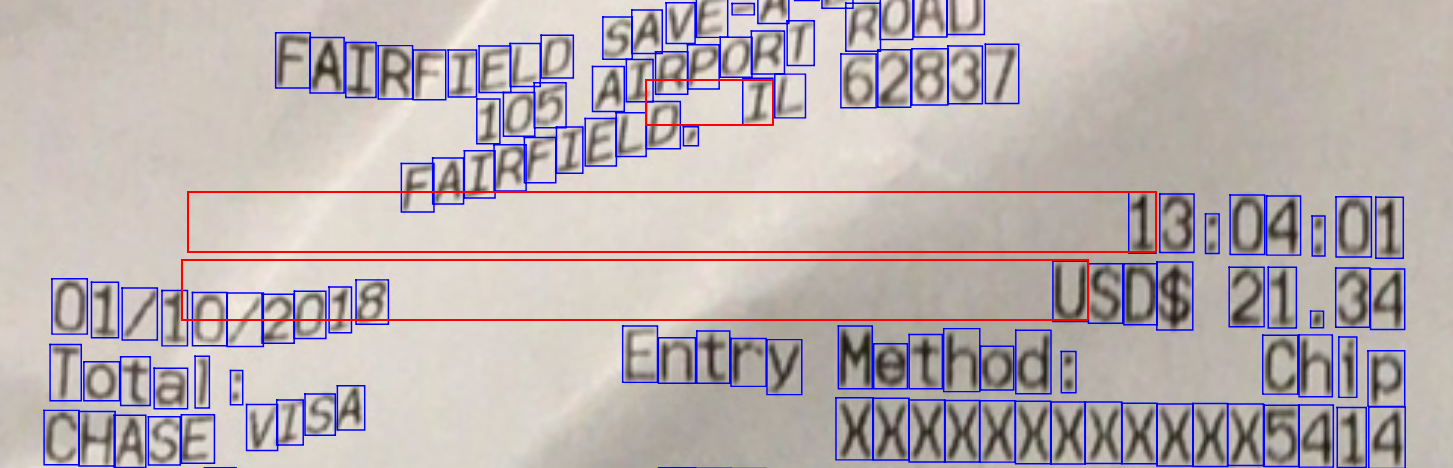
\includegraphics[width=\textwidth]{images/error-01.png}
    \caption{
        Neispavna detekcija linija u računima zbog prevelike zakrivljenosti
        sadržaja.
    }
    \label{fig:error-01}
\end{figure}

\pagebreak

\begin{figure}[!htb]
    \centering
    \captionsetup{justification=centering}
    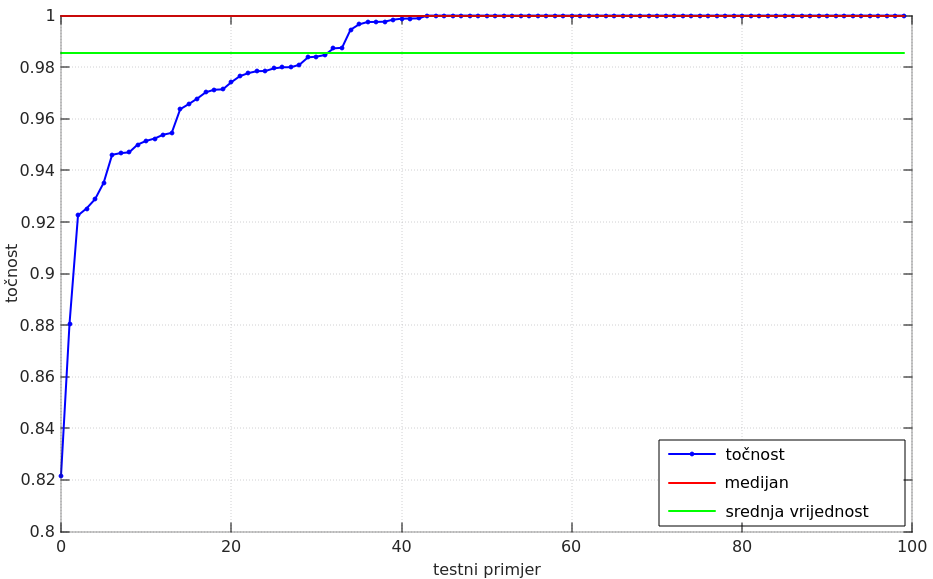
\includegraphics[width=\textwidth]{images/result-01.png}
    \caption{
        Graf točnosti algoritma za određivanje linija u sadržaju s računa iz trgovine.
    }
    \label{fig:result-01}
\end{figure}

\begin{figure}[!htb]
    \centering
    \captionsetup{justification=centering}
    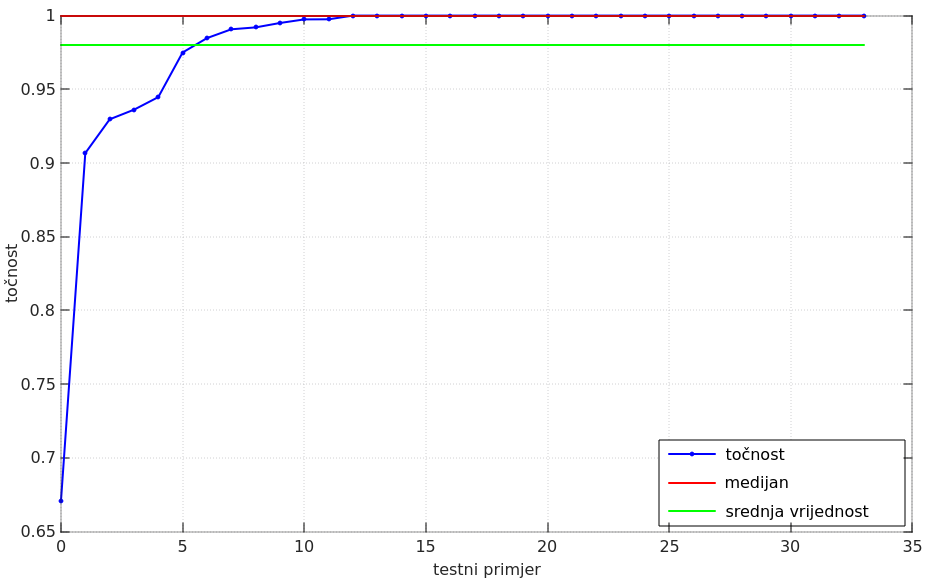
\includegraphics[width=\textwidth]{images/result-02.png}
    \caption{
        Graf točnosti algoritma za određivanje linija u sadržaju iz knjiga.
    }
    \label{fig:result-02}
\end{figure}

\pagebreak







\section{Rezultati i analiza algoritama za rastavljanje riječi}
\label{sec:rezultati-i-analiza-algoritama-za-rastavljanje-rijeci}
Slike \ref{fig:result-03} i \ref{fig:result-04} prikazuju rezultate algoritama
za rastavljanje riječi koji koriste optimalne parametre navedene u
pododjeljcima \ref{subsec:algoritam-temeljen-na-prosjecnoj-sirini znaka},
\ref{subsec:algoritam-temeljen-na-prosjecnoj-relativnoj-udaljenosti} i
\ref{subsec:algoritam-temeljen-na-prosjecnoj-udaljenosti-centara}. U tablicama
\ref{tbl:result-02} i \ref{tbl:result-03} algoritmi iz odjeljka
\ref{sec:algoritmi-za-rastavljanje-riječi} imenovani su kraticama:
\emph{avgcharwidth}, \emph{avgreldist} i \emph{avgcenterdist}. Prikazani
rezultati pokazuju točnost algoritama za rastavljanje riječi, a ujedno i
točnost cijelog sustava za određivanje strukture teksta.
Rezultati pokazuju da se s algoritmom temeljenog na prosječnoj udaljenosti
centara može potpuno točno odrediti struktura teksta, u sadržaju s računa iz
trgovina, za $54\%$ testnih primjera. Isti algoritam postiže znatno lošije
rezultate u određivanju strukture teksta u sadržaju iz knjiga.

\begin{table}[htb]
\caption{Točnost algoritama za rastavljanje riječi u sadržaju s računa iz trgovine.}
\label{tbl:result-02}
\centering
\begin{tabular}{lccccc} \hline
& Min. & Sred. & Med. & Maks. & Udio primjera s maks. točnosti \\ \hline
avgcharwidth & 0,83 & 0,98 & 0,99 & 1 & 0,34 \\
avgreldist & 0,82 & 0,98 & 0,99 & 1 & 0,33 \\
avgcenterdist & 0,83 & 0,99 & 1 & 1 & 0,54 \\ \hline
\end{tabular}
\end{table}

Ovakvi rezultati
mogu se objasniti činjenicom da je sadržaj na računima iz trgovina tiskan
fontom konstantne širine \engl{monospaced font}, i to iskorištava algoritam
\emph{avgcenterdist}. Rezultati pokazuju kako je za rastavljanje riječi u
sadržaju iz knjiga pogodnije koristiti algoritme koji se ne oslanjaju na
udaljenost centara, nego na udaljenost rubova znakova. U budućem radu trebala
bi se koristiti ta informacija kako bi se poboljšali rezultati.

\begin{table}[htb]
\caption{Točnost algoritama za rastavljanje riječi u sadržaju iz knjiga.}
\label{tbl:result-03}
\centering
\begin{tabular}{lccccc} \hline
& Min. & Sred. & Med. & Maks. & Udio primjera s maks. točnosti \\ \hline
avgcharwidth & 0,6 & 0,96 & 0,97 & 1 & 0,2 \\
avgreldist & 0,61 & 0,92 & 0,93 & 0,961436 & 0,6 \\
avgcenterdist & 0,59 & 0,93 & 0,95 & 1 & 0,02 \\ \hline
\end{tabular}
\end{table}

Najčešća pogreška koju sva tri algoritma rade je da ubacuju razmake između
znakova koji se horizontalno preklapaju (slika \ref{fig:error-02}). U budućem
radu trebao bi se uvesti mehanizam detekcije horizontalno preklapajućih znakova
koji ne bi dozvolio njihovo razdvajanje. Algoritmi također griješe u
razdvajanju uskih interpunkcijskih znakova koji su zbog svoje širine udaljeniji
od svojih susjeda u odnosu na promatrani prosjek udaljenosti ostalih znakova. U
budućem radu treba uzeti u obzir uske znakove koje ne treba razdvajati od
susjeda ako su od njih udaljeniji od nekog promatranog prosjeka.

\begin{figure}[htb]
    \centering
    \captionsetup{justification=centering,margin=2cm}
    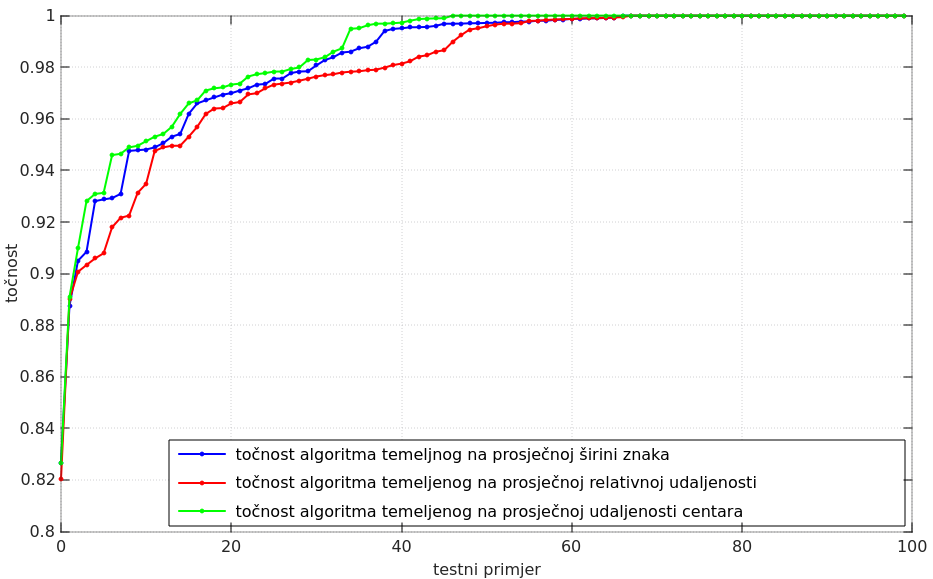
\includegraphics[width=\textwidth]{images/result-03.png}
    \caption{
        Graf točnosti algoritama za rastavljanje riječi u sadržaju s računa iz trgovine.
    }
    \label{fig:result-03}
\end{figure}

\begin{figure}[htb]
    \centering
    \captionsetup{justification=centering,margin=2cm}
    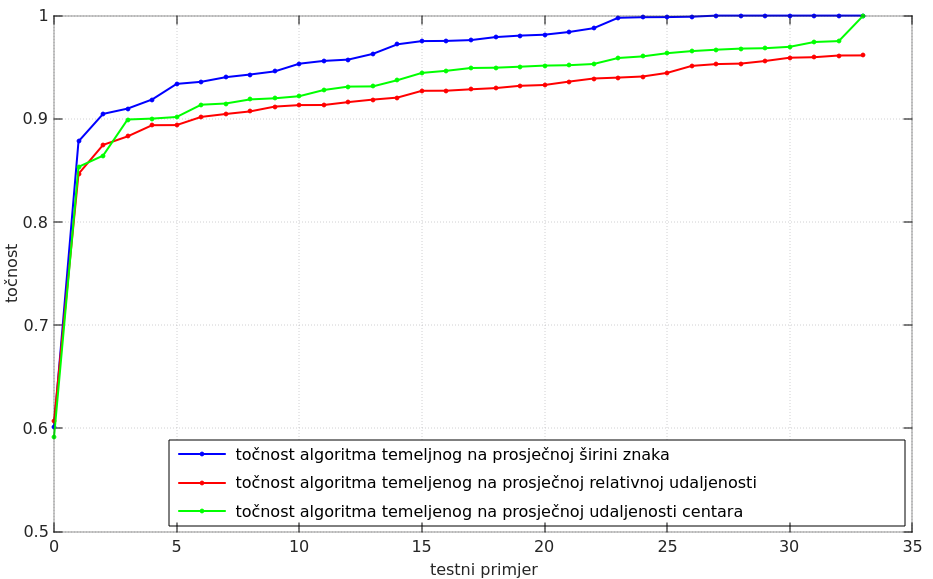
\includegraphics[width=\textwidth]{images/result-04.png}
    \caption{
        Graf točnosti algoritma za rastavljanje riječi u sadržaju iz knjiga.
    }
    \label{fig:result-04}
\end{figure}

\begin{figure}[htb]
    \centering
    \captionsetup{justification=centering,margin=2cm}
    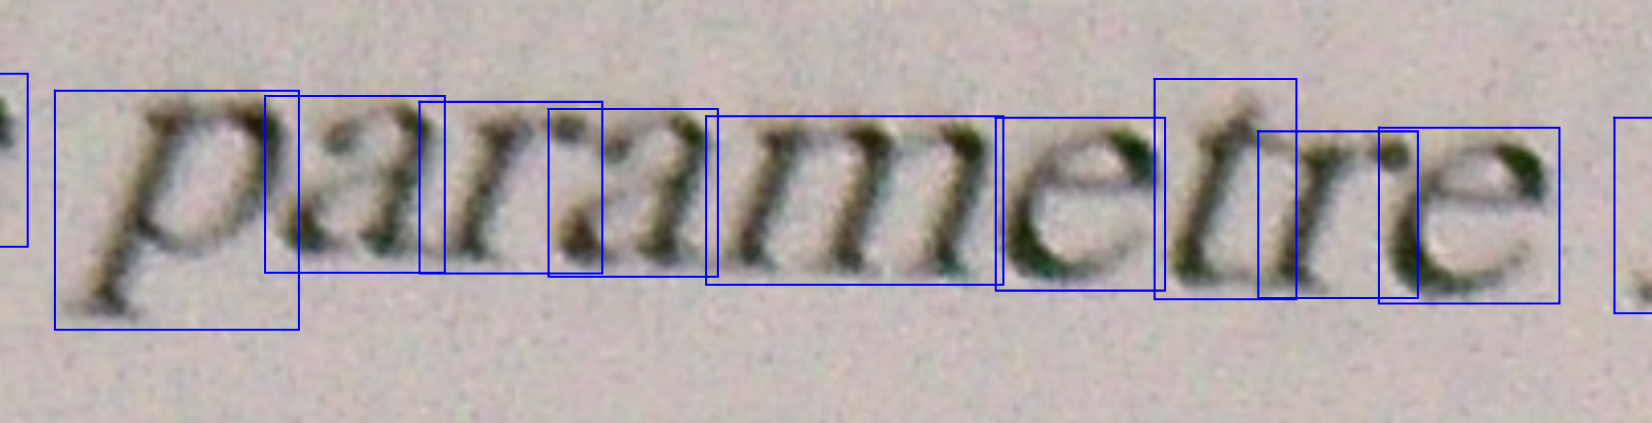
\includegraphics[width=\textwidth]{images/error-02.png}
    \caption{
        Horizontalno preklapanje znakova.
    }
    \label{fig:error-02}
\end{figure}


























\chapter{Zaključak}
Sustavi za određivanje strukture teksta sastavni su dio OCR-sustava koji se
koriste za detekciju znakova na sadržaju strukturiranom u linije, riječi i
blokove. Način izvedbe sustava ovisi o problemu koji se rješava i načinu
integracije sa OCR-sustavom. U ovom radu predstavljeni su algoritmi za
određivanje linija i razdvajanje riječi koji za određivanje
strukture koriste položaj pojedinih znakova i zajedno čine sustav za određivanje
strukture teksta.

Predstavljeni sustav za određivanje strukture teksta na temelju položaja
pojedinih znakova namjenjen je i testiran za određivanje strukture na sadržaju s
računa iz trgovina i na sadržaju iz knjiga. Rezultati i analiza pokazuju kako
postoji još prostora za poboljšanje algoritama i mjera za određivanje
točnosti. Algoritam za određivanje linija temelji se na pretpostavci da dva
susjedna znaka, koja se nalaze u istoj liniji, ostvaruju maksimalno vertikalno
preklapanje. Predstavljeni algoritmi za određivanje riječi na razne načine
koriste statističke podatke o širini i udaljenosti znakova. Dodatno,
svaki algoritam koristi parametre koji utječu na način određivanja linija i
razdvajanja riječi. Optimalni parametri algoritama ovise o problemu koji se
rješava. U ovom radu predstavljeni optimalni parametri pronađeni su ručnim
eksperimentiranjem sa skupom podataka za testiranje.

U budućem radu predlaže se sastavljanje novog skupa podataka koji bi omogućio
nezavisno testiranje dva podsustava u sustavu za određivanje strukture teksta i
predlaže se korištenje evolucijskih algoritama za pronalaženje optimalnih
parametara.

\bibliography{literatura}
\bibliographystyle{fer}

\begin{sazetak}
U ovom radu predstavljen je sustav za određivanje strukture teksta na temelju
položaja pojedinih znakova namjenjen za rješavanje problema određivanja
strukture teksta u sadržaju s računa iz trgovina i sadržaju iz knjiga. Sustav je
podjeljen na dva podsustava od kojih prvi određuje linije, a drugi rastavlja
riječi u sadržaju. Algoritam za određivanje linija temelji se na pretpostavci
da dva susjedna znaka, koja se nalaze u istoj liniji, ostvaruju maksimalno
vertikalno preklapanje. Algoritmi za rastavljanje riječi na razne načine
koriste statističke podatke o širini i udaljenosti znakova. Svaki algoritam
koristi parametre koji utječu na način određivanja linija i razdvajanja riječi


\kljucnerijeci{sustav za određivanje strukture teksta, optičko raspozavanje znakova, algoritmi za određivanje linija, algoritmi za razdvajanje riječi, segmentacija teksta, segmentacija linija}
\end{sazetak}

\engtitle{Text Layout Analysis System Based on Individual Character Positions}
\begin{abstract}
This thesis describes text layout analysis system based on individual character
positions intendend to solve the problem of determining text layout in
receipts and book content. The system is divided into two subsystems, the first
of which finds the lines in text and the other separates the words in lines.
Algorithm for finding lines in text is based on the assumption that the two
neighbouring characters in the same line have maximum vertical overlap.
Algorithms for separating the words in lines use in various ways statistics of
character width and distance of characters. Algorithms use parameters that can
be tuned and affect on how the lines are found and the words are separated.

\keywords{text layout analysis system, optical character recognition, line
finding algorithms, word separation algorithms, text segmentation, line
segmentation}
\end{abstract}

\end{document}
